\documentclass[12pt]{report}

\usepackage{setspace}
\renewcommand{\baselinestretch}{1.5}
\usepackage{float}
\usepackage{lipsum}
\usepackage{graphicx}
\usepackage[table,xcdraw,dvipsnames]{xcolor}
\usepackage{titlesec}
\usepackage{titletoc}
\usepackage{titling}
\usepackage[T1]{fontenc}
\usepackage[utf8x]{inputenc}
\usepackage{amsmath}
\usepackage{caption}
%\usepackage[a4paper,margin=0.5in]{geometry}
\usepackage[a4paper,%
            left=1cm,right=1cm,top=1cm,bottom=1cm,%
            footskip=.25in]{geometry}
\usepackage[normalem]{ulem}
\usepackage[none]{hyphenat}
\usepackage[hidelinks]{hyperref}
\useunder{\uline}{\ul}{}

% No hyphenation (word wrapping) with text justification
\tolerance=1
\emergencystretch=\maxdimen
\hyphenpenalty=10000
\hbadness=10000

% Replace table caption name
\usepackage{caption}
\captionsetup[table]{name=Tableau}

% For toc, lot and lof
\usepackage[titles]{tocloft}

% Liste des figures et les tableaux!
\graphicspath{{figures/}}
\usepackage{array}

% Disable auto indentation globally
\setlength{\parindent}{0pt}

% Choix de Font Family!
\usepackage{mathptmx}
%\usepackage{tgtermes}
%\usepackage{tgpagella}
%\usepackage{helvet}
%\usepackage{tgbonum}

% fancy logo for page numbers!
\usepackage{fancyhdr,blindtext,tikz}
\usepackage{lastpage,refcount}

% Box frame for figures #\fbox{}
\setlength{\fboxsep}{0pt}
\setlength{\fboxrule}{3pt}

% Options: Sonny, Lenny, Glenn, Conny, Rejne, Bjarne, Bjornstrup
\usepackage[Conny]{fncychap}

% Redifining from 0.1 to 1 ... 2 ... and so on
\renewcommand{\thesection}{\arabic{section}}

% Redifining from 1.1 to 1.a ... 1.b ... and so on
%\renewcommand{\thesubsection}{\alph{subsection}}

% Pour enlever les nombres dans le TOC pour les Chapitres
\titlecontents{part}[1em]
{\vskip 0.5ex\bfseries\LARGE}%
{}% numbered sections formatting
{\itshape\scshape}% unnumbered sections formatting
{}%

% Pour enlever les nombres dans le TOC pour les Chapitres
\titlecontents{chapter}[1em]
{\vskip 0.5ex\bfseries\LARGE}%
{}% numbered sections formatting
{\itshape\scshape}% unnumbered sections formatting
{\Large{\titlerule*[0.5pc]{.}}\Large{\contentspage}}%

% Pour les section aussi
\titlecontents{section}[1em]
{\vskip 0.2ex\bfseries\Large}%
{\hspace{0.15in}\contentslabel{0.13in}.\hspace{0.1in}}% numbered sections formatting
{\itshape}% unnumbered sections formatting
{\titlerule*[0.5pc]{.}\contentspage}%

% Pour les subsection
\titlecontents{subsection}[3.5em]
{\large}%
{\contentslabel{0.10in}.\hspace{0.25in}}% numbered sections formatting
{}% unnumbered sections formatting
{\titlerule*[0.3pc]{.}\contentspage}%

% Custom colors!
\definecolor{MYCOL}{HTML}{00318A}

% List of Figures settings:
\renewcommand{\listfigurename}{Liste Des Figures}
\renewcommand{\cftloftitlefont}{\vspace*{-0.6in}\hfill\color{Blue}\fontsize{35}{43}\bfseries}
\renewcommand{\cftafterloftitle}{\hfill}
\setlength{\cftfigindent}{0pt} % left aligned Fig entries
\renewcommand{\cftfigpresnum}{Figure } % put before the number
\renewcommand{\cftfigaftersnum}{:} % put before the number
\addtolength{\cftfignumwidth}{2.5em} % extra space for \cftpresnum

% List of Tables settings:
\renewcommand{\listtablename}{Liste Des Tableaux}
\renewcommand{\cftlottitlefont}{\vspace*{-0.6in}\hfill\color{Blue}\fontsize{35}{43}\bfseries}
\renewcommand{\cftafterlottitle}{\hfill}
\setlength{\cfttabindent}{0pt} % left aligned Tab entries
\renewcommand{\cfttabpresnum}{Tableau } % put before the number
\renewcommand{\cfttabaftersnum}{:} % put before the number
\addtolength{\cfttabnumwidth}{2.5em} % extra space for \cftpresnum

% Table of contents settings:
\renewcommand{\contentsname}{Table Des Matières}

\usepackage[framemethod=TikZ]{mdframed}

% Pour la box de Th\`eme!
\mdfdefinestyle{MyFrame}{%
    linecolor=black,
    outerlinewidth=6pt,
    roundcorner=12pt,
    innertopmargin=13pt,
    innerbottommargin=13pt,
    innerrightmargin=20pt,
    innerleftmargin=20pt,
    backgroundcolor=gray!30!white}


% My custom page style
\fancypagestyle{myfancy}{%   
   \fancyhf{}%
   \fancyfoot[C]{\tikz[baseline={(0,0)},anchor=center] \node[label={center:\thepage}]{
\includegraphics[scale=.037]{../Icon/cloud.png}};}%
   \renewcommand{\headrulewidth}{0pt}%
   \renewcommand{\footrulewidth}{0pt}%
   \fancyhead{}
   \fancyfoot{}
   \fancyfoot[C]{\vspace{-0.35in}\textcolor{Gray}{\Large{Page}}\hspace{0.04in} \large{\thepage}\hspace{0.07in}\large{|}\hspace{0.07in}\large{72}}%\pageref{LastPage}}}
}%
\pagestyle{empty}

% Custom environment
\newenvironment{changemargin}[2]{%
\begin{list}{}{%
\setlength{\topsep}{0pt}%
\setlength{\leftmargin}{#1}%
\setlength{\rightmargin}{#2}%
\setlength{\listparindent}{\parindent}%
\setlength{\itemindent}{\parindent}%
\setlength{\parsep}{\parskip}%
}%
\item[]}{\end{list}}

% 'myfancy' page styling is also applied on chapters!
\usepackage{etoolbox}
\patchcmd{\chapter}{\thispagestyle{empty}}{\thispagestyle{myfancy}}{}{}

\titleformat{\chapter}
{\centering\fontsize{40}{50}\bfseries\color{Blue}\scshape}
{}
{}
{\vspace{-1.7in}{\color{Blue} \rule{\linewidth}{1.2mm} }}[\vspace{-0.35in}{\color{Blue} \rule{\linewidth}{1.2mm} }\vspace{-1in}]

\titleformat{\section}
{\Large\bfseries\color{MidnightBlue}}
{\thesection.\hspace{0.08in}}
{0em}
{}[\titlerule]

\titleformat{\subsection}
{\large\bfseries\color{RoyalBlue}}
{\hspace{0.25in}\thesubsection\hspace{0.08in}}
{0em}
{}[]

\titleformat{\subsubsection}
{\bfseries}
{\hspace{0.40in}}
{0em}
{}[]

\newenvironment{myindentpar}[1]%
  {\begin{list}{}%
          {\setlength{\leftmargin}{#1}}%
          \item[]%
  }
  {\end{list}}

\usepackage{tikz}
\usetikzlibrary{calc}

\begin{document}

\begin{titlepage}

   \begin{tikzpicture}[remember picture, overlay]
      \draw[line width = 2pt] ($(current page.north west) + (0.25in,-0.25in)$) rectangle ($(current page.south east) + (-0.25in,0.25in)$);
   \end{tikzpicture}

   \begin{center}
       \vspace*{-0.4in}

       \begin{large}

           \textbf{R}épublique \textbf{A}lgérienne \textbf{D}émocratique et \textbf{P}opulaire

           \textbf{M}inistère de l'\textbf{E}nseignement \textbf{S}upérieur et de la \textbf{R}echerche \textbf{S}cientifique

           \textbf{U}niversité \textbf{M}'Hamed \textbf{B}ougara de \textbf{B}oumerdès

       \end{large}

       \vspace{0.1in}

       \begin{figure}[h]
       \hspace{0.29in}
           \Large{Faculté des Sciences}$
       \hspace{0.25in}
       \begin{array}{l}
       \centering
           
\includegraphics[width = 2.2in, height = 1.4in]{../Images/UnivUMBB.jpg}
       \end{array}
       \hspace{-0.2in}
           $\Large{Département d'informatique}
       \hspace{-0.8in}
       \end{figure}
   \end{center}

    \hspace{0.2in}
    \large{\textbf{Domaine \,\; :}  Mathématiques Informatique}
    \kern 1in
    \large{\textbf{Année universitaire :}}

    \hspace{0.2in}
    \large{\textbf{Filière \quad\,\,\, :}  Informatique}
    \kern 2.65in
    2019 / 2020

    \hspace{0.2in}
    \large{\textbf{Spécialité \, :}  Informatique}

    \hspace{0.2in}
    \Large{N°de l’Arrêté d’habilitation de la spécialité : arrêté n °872 du 26/07/2016}

    \begin{center}
        \begin{large}

            \textit{\textbf{\uline{Mémoire de fin d'études en vu de l'obtention du}}}
        
            \textit{\textbf{\uline{Diplôme de Licence Académique}}}

        \end{large}

        \vspace{0.2in}

        \textit{\Huge{\textbf{\uline{Thème}}}}

        \begin{mdframed}[style=MyFrame]
            \begin{center}
            \color{BlueViolet}
              \LARGE{\textbf{La réalisation d'un tableau de bord pour le suivi}}

              \LARGE{\textbf{des recours des étudiants du département}}
            \end{center}
        \end{mdframed}
    \end{center}

    \vspace{-0.05in}

    \hspace{0.2in}
    \textit{\textbf{Présenté par :}}

    \hspace{0.2in}
    Neggazi Mohamed Lamine

    \hspace{0.2in}
    Taleb Zineb

    \begin{center}
        \vspace{-0.1in}
        \textit{\textbf{Soutenu le ... / ... / 2020 Devant le jury composé de}}\\
        \hspace{1.867in}
        \qquad :\qquad Examinateur\\
        Yahiatene Youcef\qquad :\qquad Encadreur
    \end{center}


\end{titlepage}

\newpage

\vspace*{0.1in}

\thispagestyle{empty}

\let\clearpage\relax
% New margins for rest of document
\newgeometry{left=2.4cm,right=1.7cm,top=1cm,bottom=1cm,nohead}

\begin{center}
    \textit{\fontsize{34}{46}{\bfseries{\color{Blue}{Dédicace}}}}
    \\
    \vspace{0.2in}
    %\color{Red}{\large\textbf{{\lipsum[1-2]}}}
    % Taleb Zineb
    \itshape
    \Large{\underline{Je dédie ce travail a :}}\\          \textbf{\large{À mon cher père Abd laziz,}}\\\vspace{-0.1in}
    \textbf{\large{À ma chère mère Zohra,}}\\
    \large{Qui n'ont jamais cessé, de formuler des prières à mon égard, de me soutenir\\\vspace{-0.1in}et de m'épauler pour que je puisse atteindre mes objectifs.}\\
    \textbf{\large{À mes deux chères sœurs Asma et Amel,}}\\
    \large{Pour leur soutien et leurs conseils précieux tout aux long de mes études.}\\
    \textbf{\large{À mes chers amis et mon binôme Amine,}}\\
    \large{Pour leur aide et supporte dans les moments difficiles.}\\
    \textbf{\large{À toute ma famille, À tous ceux que j’aime.}}\\\vspace{0.1in}
    \hfill\textbf{\Large{Taleb Zineb}}

    \vspace{0.2in}
    %\color{Red}{\large\textbf{{\lipsum[1-2]}}}
    % Neggazi Amine
    \itshape
    \Large{\underline{Je dédie ce travail a :}}\\          \textbf{\large{À mon cher père Khelifa,}}\\\vspace{-0.1in}
    \textbf{\large{À ma chère mère Fatma Zohra,}}\\
    \large{Aucun hommage ne pourrait être a la hauteur de l’amour et de soutien\\\vspace{-0.1in}dont ils ne cessent de me combler,}\\
    \textbf{\large{À ma chère sœur Maria,}}\\
    \large{Pour son soutien et ces conseils précieux tout aux longue de mes études.}\\
    \textbf{\large{À mes chers amis et mon binôme Zineb,}}\\
    \large{Pour leur aide et supporte dans les moments difficiles.}\\
    \textbf{\large{À toute ma famille, À tous ceux que j’aime.}}\\\vspace{0.1in}
    \hfill\textbf{\Large{Neggazi Mohamed Lamine}}

\end{center}

%\addcontentsline{toc}{chapter}{\vspace{-0.12in}\color{Blue}{Dédicace}}
\cftaddtitleline{toc}{part}{\vspace{-0.12in}\color{Blue}{Dédicace}}{}

\newpage

\vspace*{0.5in}

\thispagestyle{empty}

\begin{center}
    \textit{\fontsize{34}{46}{\bfseries{\color{Blue}{Remerciement}}}}
    \vspace{0.7in}
    \textit{
    \\\Large{<< Nous tenons tout d’abord à remercier Dieu de nous avoir donné le courage et la patience pour accomplir ce travail >>}
    \vspace{0.4in}
    \\\Large{<< Nous tenons à exprimer notre grand remerciement à nos très chers parents pour leur soutien moral et leur encouragement >>}
    \vspace{0.4in}
    \\\Large{<< Nous adressons nos sincères remerciements à Monsieur Youcef Yahiatene qui nous a confié ce sujet et qui a assumé l’encadrement de notre projet, l’intérêt qu’il a porté à notre travail, sa bienveillance, sa rigueur scientifique, ses hautes qualités humaines, ont constitué une aide précieuse et nous a permis de mener à terme ce travail >>}
    \vspace{0.4in}
    \\\Large{<< Enfin, mes remerciements s’adressent aussi à tous ceux qui ont participé, de près ou de loin, à l’élaboration de ce projet de fin d’études et en particulier à ma famille et mes amis >>}
    \\}
\end{center}
\cftaddtitleline{toc}{part}{\vspace{-0.12in}\color{Blue}{Remerciement}}{}

\newpage

\vspace*{0.2in}

\thispagestyle{empty}

\begin{center}
    {\color{Blue} \rule{3in}{1.4mm} }\\
    \vspace{0.1in}
    \scshape{\fontsize{34}{46}{\bfseries{\color{Blue}{Résumé}}}}
    \\
    \vspace{0.6in}
\end{center}
\cftaddtitleline{toc}{part}{\vspace{-0.12in}\color{Blue}{Résumé}}{}
\begin{changemargin}{0.9cm}{0.9cm}
Les universités contemporaines reçoivent beaucoup d’informations et de données concernant les étudiants et les employés, pour les traiter et faire des statistiques durant toute l’année scolaire, prenant par exemple les dossiers de recours, ils occupent un énorme espace dans la base de données de la faculté, ces derniers changent quotidiennement et on a besoin de ces statistique après chaque modification.
\\\\
Notre objectif est de créer un tableau de bord qui consiste en l'organisation de plusieurs indicateurs de sa performance, il est efficace d’avoir une vue en temps réel ou différé des enjeux de son activité et de permettre la visualisation de données brutes.
\\\\
Aussi l’agrégation de données clés permettant de gagner en efficacité et de prendre les meilleures décisions. Le tableau de bord confirme de façon structurée les impressions et  indique la nécessité d’entreprendre une analyse plus approfondie, en cernant la zone à problème, il oriente des corrections à mener avant d’agir. le tableau de bord est utilise aussi afin de permettre la visualisation de données qui rendre les données plus accessibles et compréhensibles, elle donne du sens à ces données.
\\\\
Pour cela, elle fait appel à différentes représentations visuelles pour la faciliter de comprendre la base de données avec des représentation graphique en deux ou trois dimensions, utilisant des couleurs et des trames qui permettent d'éclaircir la lecture des données de manière plus simple.
\end{changemargin}

\vspace{1in}

\begin{changemargin}{0.9cm}{0.9cm}
Mots clés : recours, tableau de bord, visualisation de données, représentation graphique.
\end{changemargin}

\newpage

\vspace*{0.2in}

\thispagestyle{empty}

\begin{center}
    {\color{Blue} \rule{3in}{1.4mm} }\\
    \vspace{0.1in}
    \scshape{\fontsize{34}{46}{\bfseries{\color{Blue}{Abstract}}}}
    \\
    \vspace{0.6in}
\end{center}
\cftaddtitleline{toc}{part}{\vspace{-0.12in}\color{Blue}{Abstract}}{}
\begin{changemargin}{0.9cm}{0.9cm}
Contemporary universities receive a lot of information and data concerning students and employees, to process them and make statistics throughout the school year, taking for example the files of recourses, they occupy a huge space in the database of the faculty, these change daily and we need these statistics after each modification.
\\\\
Our goal is to create a dashboard that consists of the organization of several performance indicators, it is effective to have a real-time or deferred view of the challenges of your activity and to allow the visualization of raw data.
\\\\
Also the aggregation of key data to gain efficiency and make the best decisions. The dashboard confirms impressions in a structured way and indicates the need for a more in-depth analysis, by identifying the problem area, it directs corrections to be made before acting. the dashboard is also used to allow data visualization which makes data more accessible and understandable, it gives meaning to this data.
\\\\
To do this, it uses different visual representations to make it easier to understand the database with two or three-dimensional graphical representations, using colors and frames that make it easier to read the data.
\end{changemargin}

\vspace{1in}

\begin{changemargin}{0.9cm}{0.9cm}
Keywords : recourses, dashboard, data visualization, graphical representations.
\end{changemargin}

\newpage

\cftaddtitleline{toc}{part}{\vspace{-0.12in}\color{Blue}{Table des matières}}{}
\tableofcontents

\newpage

\cftaddtitleline{toc}{part}{\vspace{-0.12in}\color{Blue}{Liste des figures}}{}
\listoffigures

\newpage

\cftaddtitleline{toc}{part}{\vspace{-0.12in}\color{Blue}{Liste des tableaux}}{}
\listoftables

\addtocontents{toc}{\protect\renewcommand{\protect\cftsecleader}{\protect\cftdotfill{\protect\cftsecdotsep}}}

\addtocontents{lof}{\protect\thispagestyle{empty}}
\addtocontents{lot}{\protect\thispagestyle{empty}}
\addtocontents{toc}{\protect\thispagestyle{empty}}

\newpage

\pagestyle{myfancy}

\vspace*{-0.2in}

\setcounter{page}{1}

\begin{center}
    {\color{Blue} \rule{6.2in}{1.4mm} }\\
    \vspace{0.1in}
    \scshape{\fontsize{34}{46}{\bfseries{\color{Blue}{Introduction générale}}}}
    \\
    \vspace{0.5in}
\end{center}
\addcontentsline{toc}{chapter}{\vspace{-0.12in}\color{Blue}{Introduction générale}}
De nos jours, une bonne partie de la population mondiale utilise internet. Le Web est accessible de partout et tout le temps, un site Web est une véritable vitrine virtuelle qui permet d’être visible sur le net et de communiquer en temps réel, C’est un investissement et non une dépense qui facilite la vie des gens, le développement Web réponde aux attentes grandissantes des utilisateurs, et aux tendances en matière de conception, il est amené à maîtriser de multiples outils et technologies au sein de projets parfois très différents. Que ce soit en équipe ou en freelance.
\\\\
\uline{Problématique :} parmi les choses que nous aimerions changer, nous parlons de la manière actuelle de soumettre des recours qui consiste à écrire le recours dans un papier ou en utilisant Google Forms, puis à soumettre le recours pour le traiter, le problème de cette solution est le grand espace mémoire qui occupe la base de données, la perte de données à cause de la dégradation du papier et le traitement prend beaucoup de temps.
\\\\
Nous avons proposé une solution qui est la création d'un site internet qui contient un tableau de bord pour le suivi des recours des étudiants dans le département informatique, elle est adaptée pour réserver des espaces, un espace dédié aux étudiants et un autre dédié à l'administration, et aussi aux enseignants afin qu'ils peut refuser ou valider les recours.
\\\\
Dans le but de bien présenter notre travail, nous avons divisé notre mémoire en trois chapitre :
\\
\uline{Le premier chapitre :} englobe une étude générale sur notre projet, plus précisément une partie de développement Web, et une autre qui fait une étude sur la gestion et les statistiques des recours.
\\
\uline{Le deuxième chapitre :} 
Dans cette partie, nous allons présenter l'analyse et la conception de notre solution, nous allons détails quelques diagrammes à savoir : Cas d'utilisation, Séquence, Activité,  Déploiement et de classes.
\\
\uline{Le troisième chapitre :} qui est composé de deux parties la partie réalisation (les langages de programmation et les outils utilisés), et la partie implémentation qui est en plusieurs étapes, elle consiste à créer une page de connexion et d'inscription, ainsi qu'ajouter des styles et des interactions à l'aide de nombreuses technologies, et plus de fonctionnalités qui consistent à télécharger des fichiers et des photos de profil et tant de mesures de sécurité.

\newpage

\vspace*{-0.2in}

\begin{center}
    {\color{Blue} \rule{6.2in}{1.4mm} }\\
    \vspace{0.1in}
    \scshape{\fontsize{34}{46}{\bfseries{\color{Blue}{Planification}}}}
    \\
    \vspace{0.12in}
\end{center}
\addcontentsline{toc}{chapter}{\vspace{-0.12in}\color{Blue}{Planification}}
\hspace*{-0.05in}
Dans cette partie, nous avons fait la planification de notre projet pour savoir qui fait quoi et faire une répartition des tâches. Cette planification consiste en un diagramme de Gantt et de réseau (utilisé en ordonnancement et en gestion de projet et permettant de visualiser dans le temps les diverses tâches composant un projet), nous avons pris 15 jours de confinement à cause de covid-19 et quelques jours fériés, d'anniversaires et l'eid el adha...
\\
\textbf{\underline{Note :}} Nous avons utilisé ProjectLibre pour établir ces différents schémas.
\\
Nous avons essayé de faire certaines tâches simultanément comme indiqué ci-dessous :

\vspace{0.15in}

\begin{figure}[h]
\centering
    \fbox{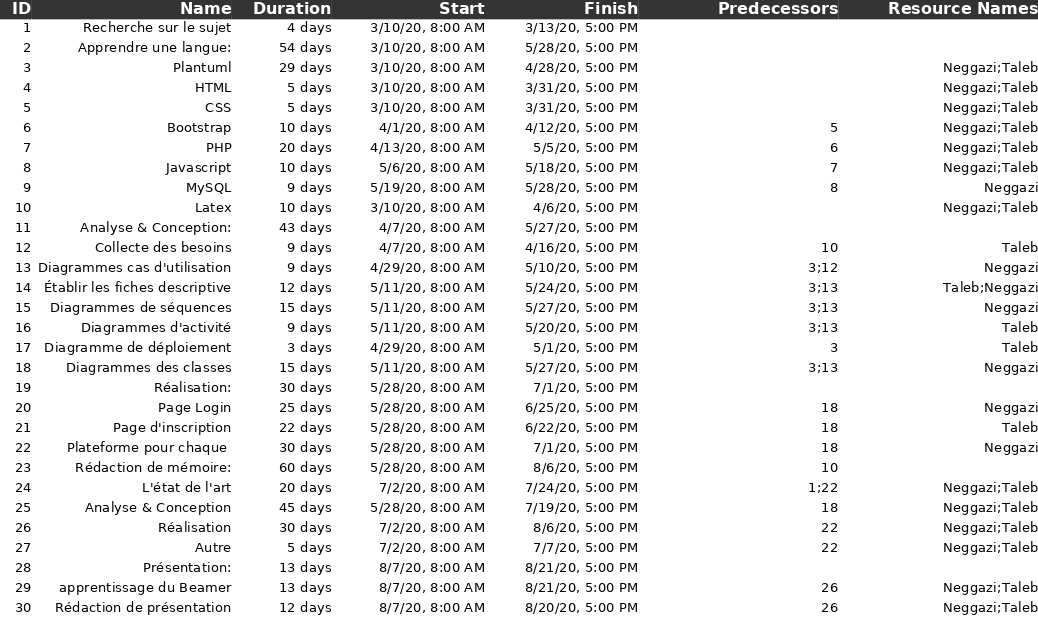
\includegraphics[width = 6.6in, height = 6.2in]{../Planification/Tasks.png}}
\caption{Les Tâches}
\end{figure}

\newpage

\begin{figure}[H]
\centering
    \fbox{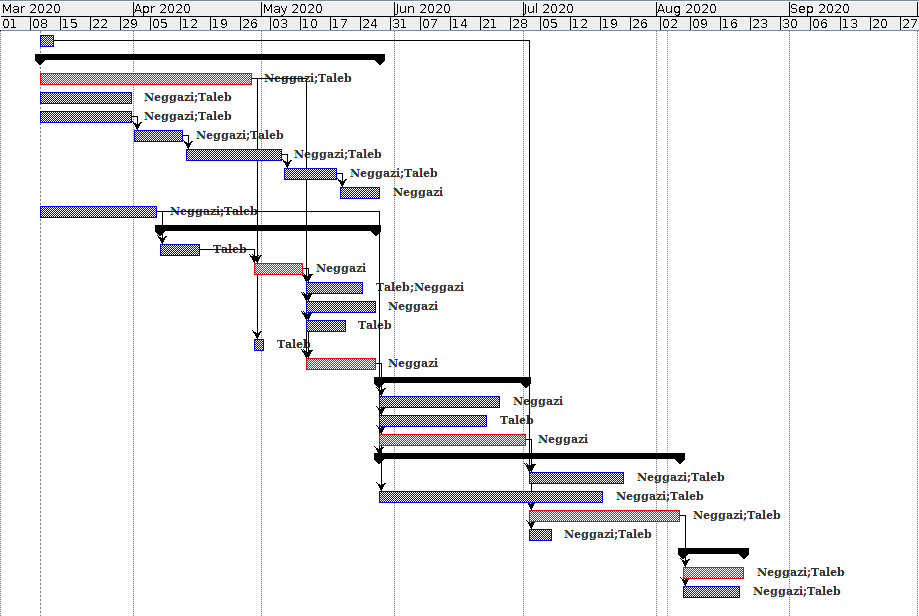
\includegraphics[width = 9in, height = 6.6in, angle = -90]{../Planification/Gantt.png}}
\caption{Diagramme de Gantt}
\end{figure}

\newpage

\begin{figure}[H]
\centering
    \fbox{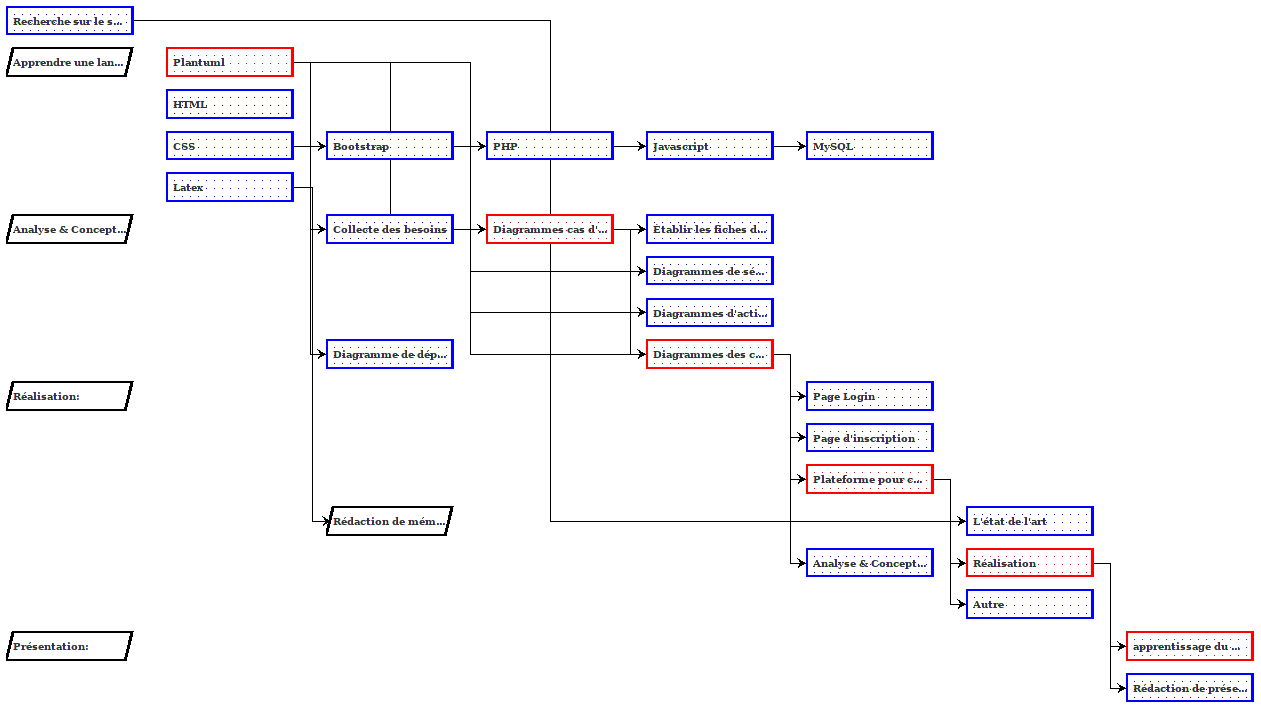
\includegraphics[width = 9in, height = 6.6in, angle = -90]{../Planification/Network.png}}
\caption{Diagramme de réseau}
\end{figure}

\newpage

\vspace*{\fill}
\begin{center}
    {\color{Blue} \rule{\linewidth}{1.2mm} }\\
\vspace{0.25in}
 {\centering\fontsize{30}{40}{\bfseries{\color{Blue}{\scshape{Chapitre I : Étude Général}}}}}
\vspace{0.35in}\\
    {\color{Blue} \rule{\linewidth}{1.2mm} }
\end{center}
\vspace*{\fill}
\addcontentsline{toc}{chapter}{\color{Blue}{Chapitre I : Étude Général}}
\setcounter{section}{0}

\newpage

\section{Introduction}
\vspace{0.2in}
Les universités de nos jours font face à des problèmes en ce qui concerne les recours universitaires, dans cette partie, nous aborderons une idée générale sur le développement Web, ainsi qu'une étude sur la gestion des recours des étudiants avec des exemples de notre faculté des sciences, par la suite, nous allons établir les points forts et les points faibles de la solution actuelle, un brainstorming avec les étudiants pour savoir comment ils souhaitent voir le traitement des recours, donner une proposition  qui pourra répondre le plus aux besoins de notre université, nous verrons aussi une explication de cette solution avec les détails nécessaires.

\vspace{0.7in}

%\begin{figure}[h]
%\centering
%    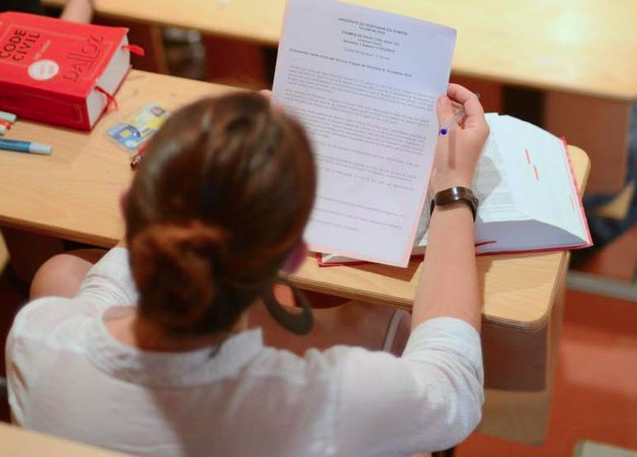
\includegraphics[width = 6.6in, height = 4.4in]{../Images/Recours.png}
%\caption{Feuille d'examen}
%\end{figure}

\newpage

\section{Le développement Web}
\vspace{0.2in}
Le développement Web est le travail impliqué dans le développement d'un site Web pour Internet (World Wide Web) ou un intranet (un réseau privé). Le développement Web peut aller du développement d'une simple page statique unique de texte brut à des applications Internet complexes (applications Web), des entreprises électroniques et des services de réseaux sociaux. Une liste plus complète de tâches auxquelles le développement Web se réfère généralement peut inclure l'ingénierie Web, la conception Web, le développement de contenu Web, la liaison client, les scripts côtés clients / côtés serveur, la configuration de la sécurité du serveur Web et du réseau et le développement du commerce électronique.
\\\\
Chez les professionnels du Web, le «développement Web» fait généralement référence aux principaux aspects non liés à la conception de la création de sites Web : l'écriture de balisage et le codage. Le développement Web peut utiliser des systèmes de gestion de contenu (CMS) pour rendre les modifications de contenu plus faciles et disponibles avec des compétences techniques de base.

\vspace{0.6in}

\begin{figure}[h]
\centering
    
\includegraphics[width = 6.6in, height = 3.8in]{../Images/webDev.jpeg}
\caption{Développement Web}
\end{figure}

\newpage

\section{Outils de développement Web}
\vspace{0.2in}
Les outils de développement Web (souvent appelés devtools) permettent aux développeurs Web de tester et de déboguer leur code. Ils diffèrent des créateurs de sites Web et des environnements de développement intégrés (IDE) en ce qu'ils ne facilitent pas la création directe d'une page Web, mais plutôt des outils utilisés pour tester l'interface utilisateur d'un site Web ou d'une application Web.
\\\\
Les outils de développement Web sont des modules complémentaires de navigateur ou des fonctionnalités intégrées dans les navigateurs Web. Les navigateurs Web les plus populaires, tels que Google Chrome, Firefox, Internet Explorer, Safari et Opera, ont des outils intégrés pour aider les développeurs Web, et de nombreux modules complémentaires peuvent être trouvés dans leurs centres de téléchargement de plugins respectifs.
\\\\
Les outils de développement Web permettent aux développeurs de travailler avec diverses technologies Web, notamment HTML, CSS, DOM, JavaScript et d'autres composants gérés par le navigateur Web. En raison de la demande croissante des navigateurs Web pour en faire plus, les navigateurs Web populaires ont inclus plus de fonctionnalités destinées aux développeurs.
\\\\
Nous allons utiliser la plupart des outils listés ci-dessus.
\\
Voici quelques-uns des plus basiques :

\vspace{0.2in}

\begin{figure}[h]
\centering
    
\includegraphics[width = 6in, height = 2.7in]{../Images/webDevTools.jpg}
\caption{Outils de Développement Web}
\end{figure}

\newpage

\section{Étude sur la gestion des recours}
\vspace{0.2in}
Un étudiant, durant son parcours, peut rencontrer des événements (souci d’une note) qui l'amèneront à effectuer des démarches exceptionnelles, faire un recours par exemple.

\subsection{C'est quoi un recours?}
D'une manière générale un recours est le fait d'en appeler à une tierce personne ou à une institution, pour obtenir la reconnaissance d'un droit qui a été méconnu.

\subsection{Modèle d’un recours}
\vspace{0.1in}
Lettre pour signaler une erreur sur le relevé de notes et demander une rectification. <<Figure 7>>

\vspace{0.2in}

\begin{figure}[h]
\centering
    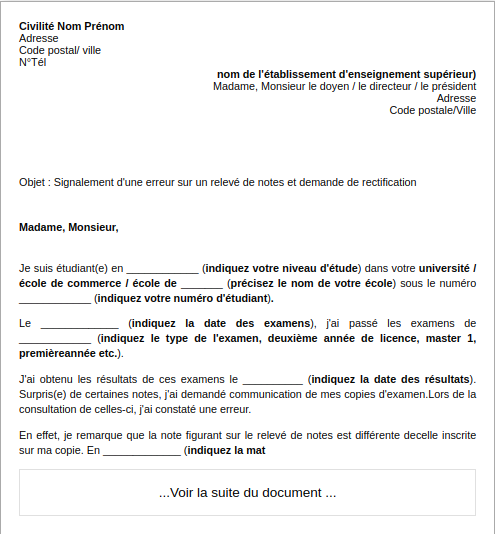
\includegraphics[width = 6in, height = 5.5in]{../Images/ModeleRecours.png}
\caption{Modèle d’un recours}
\end{figure}

\newpage

\section{La solution actuelle}
Il existe deux façons de déposer un recours dans notre faculté (la faculté des sciences / université de boumerdes) :
\begin{itemize}
    \item La première est d'écrire le recours dans une feuille (le modèle de recours en haut) où l'on explique le problème avec les informations nécessaires (matricule, nom, prénom, module, l'enseignant...).\\Ensuite, soumettre le recours au département pour le traiter.
    \item La deuxième façon est avec Google Forms, Vous devez d'abord remplir les informations nécessaires.\\Ensuite, sélectionner les unités dans les quelles vous avez un problème et enfin, soumettez le recours pour le traiter.
\end{itemize}

\subsection{Les points forts}
\begin{itemize}
    \item La communication directe avec l'administration.
    \item L'étudiant peut bien expliquer le problème qui la conduit à faire le recours. 
\end{itemize}

\subsection{Les points faibles}
\begin{itemize}
    \item La présence obligatoire d'étudiant pour soumettre son recours.
    \item Occupe beaucoup d'espace mémoire dans la base de données.
    \item Perte de données en raison de la dégradation du papier.
    \item Ça prend beaucoup de temps (pour écrire le recours...).
\end{itemize}

\section{Le brainstorming}

\subsection{Introduction}
Le brainstorming consiste à rassembler un groupe de personnes choisies à qui l’on demande d’exprimer librement leurs idées, qui seront, par la suite analysées et classées, le but du brainstorming est de maximiser les idées, les propositions et de solutions sur un sujet donné.

\subsection{Les règles du brainstorming}

\newpage

\begin{table}[h]
\centering
\large
\resizebox{\textwidth}{!}{%
\begin{tabular}{|l|l|}
\hline
\rowcolor[HTML]{ECF4FF}
\multicolumn{1}{|c|}{\cellcolor[HTML]{ECF4FF}{\color[HTML]{000000} {\ul \textbf{À ne pas faire :}}}} &
  \multicolumn{1}{c|}{\cellcolor[HTML]{ECF4FF}{\color[HTML]{000000} {\ul \textbf{À faire :}}}} \\ \hline
\rowcolor[HTML]{DAE8FC}
{\color[HTML]{000000} - Impliquer immédiatement tout le monde.}           & {\color[HTML]{000000} - Donnez aux gens le temps de réfléchir.}                 \\ \hline
\rowcolor[HTML]{ECF4FF}
{\color[HTML]{000000} - Mettre des limites à la séance de brainstorming.} & {\color[HTML]{000000} - Laisser les gens s'exprimer librement sans contrainte.} \\ \hline
\rowcolor[HTML]{DAE8FC}
{\color[HTML]{000000} - Rejeter des idées sur le coup.}                   & {\color[HTML]{000000} - S'assurer que tout le monde partage au moins une idée.} \\ \hline
\rowcolor[HTML]{ECF4FF}
{\color[HTML]{000000} - Se concentrer sur la qualité des idées.}          & {\color[HTML]{000000} - Tabler sur la quantité d'idées.}                        \\ \hline
\rowcolor[HTML]{DAE8FC}
{\color[HTML]{000000} - Annoter uniquement les bonnes idées.}             & {\color[HTML]{000000} - Tout annoter.}                                          \\ \hline
\rowcolor[HTML]{ECF4FF}
{\color[HTML]{000000} \begin{tabular}[c]{@{}l@{}}- Limiter la génération d'idées à une seule\\ séance de brainstorming.\end{tabular}} &
  {\color[HTML]{000000} \begin{tabular}[c]{@{}l@{}}- Permettre aux gens d'ajouter des idées dans un\\ deuxième temps.\end{tabular}} \\ \hline
\end{tabular}%
}
\caption{Règles de brainstorming}
\end{table}

\subsection{Le brainstorming avec les étudiants}

Voici quelques idées du résultat de brainstorming des étudiants de la faculté des sciences :
\begin{itemize}
    \item Développer le site Web de la faculté et faire une partie liée aux recours.
    \item Créer un site Web spécial aux recours.
    \item Créer un espace administratif dédié spécialement aux recours.
    \item Faire des réunions pour traiter les recours.
    \item Faire un lien où on peut envoyer des fichiers pour justifier l'erreur.
\end{itemize}

\section{La solution proposée}
La réalisation d’un tableau de bord pour le suivi des recours des étudiants du département d’informatique. Dans la solution que nous avons proposée, nous avons un espace dédié aux :
\begin{itemize}
    \item Étudiants pour soumettez leur recours.
    \item Edministrations pour gérer les recours.
    \item Enseignants afin qu’ils puissent traiter les recours.
\end{itemize}

\section{Conclusion}
Dans ce chapitre, nous avons présenté le problème de la solution actuelle avec ses détails concernant la gestion des recours, et nous avons proposé un site internet avec un tableau de bord après avoir analysé les résultats de notre brainstorming, cette solution va être mise en œuvre dans les prochains chapitres.

\newpage

\vspace*{\fill}
\begin{center}
    {\color{Blue} \rule{\linewidth}{1.2mm} }\\
\vspace{0.25in}
    {\centering\fontsize{30}{40}{\bfseries{\color{Blue}{\scshape{Chapitre II : Analyse \& Conception}}}}}
\vspace{0.35in}\\
    {\color{Blue} \rule{\linewidth}{1.2mm} }
\end{center}
\vspace*{\fill}
\addcontentsline{toc}{chapter}{\color{Blue}{Chapitre II : Analyse \& Conception}}
\setcounter{section}{0}

\newpage

\section{Introduction}
\vspace{0.2in}
\uline{L'analyse :} Plutôt que d’apporter une solution, elle met l’accent sur une enquête par rapport à un problème et sur des besoins. Par exemple, si l’on souhaite informatiser le système d’information d’une bibliothèque, comment s’y prendrait-on?
\\
Le mot <<Analyse>> est un terme général, de manière plus précise on pourrait parler, d’analyse des besoins (une enquête sur les besoins) ou de l’analyse des objets (une enquête sur les objets du domaine).
\\
\uline{Conception :} La conception apporte une solution théorique aux exigences, mais n’engage pas la mise en œuvre. Par exemple, la conception peut produire une description d’un schéma de base de données et des objets logiciels. Au bout du compte, c’est probable que les résultats de la conception seront mises en œuvre.

\vspace{-0.1in}

\subsection{Objectifs de l’analyse}
\begin{itemize}
    \item Étude du m\'etier du client.
    \item Étude des besoins des utilisateurs.
    \item Reformulation du cahier des charges sous une forme exploitable en conception.
\end{itemize}

\vspace{-0.15in}

\subsection{Objectifs de la conception}
\begin{itemize}
    \item D\'efinition de l’architecture logicielle.
    \item D\'efinition du comportement de l’application.
\end{itemize}

\begin{figure}[h]
\centering
    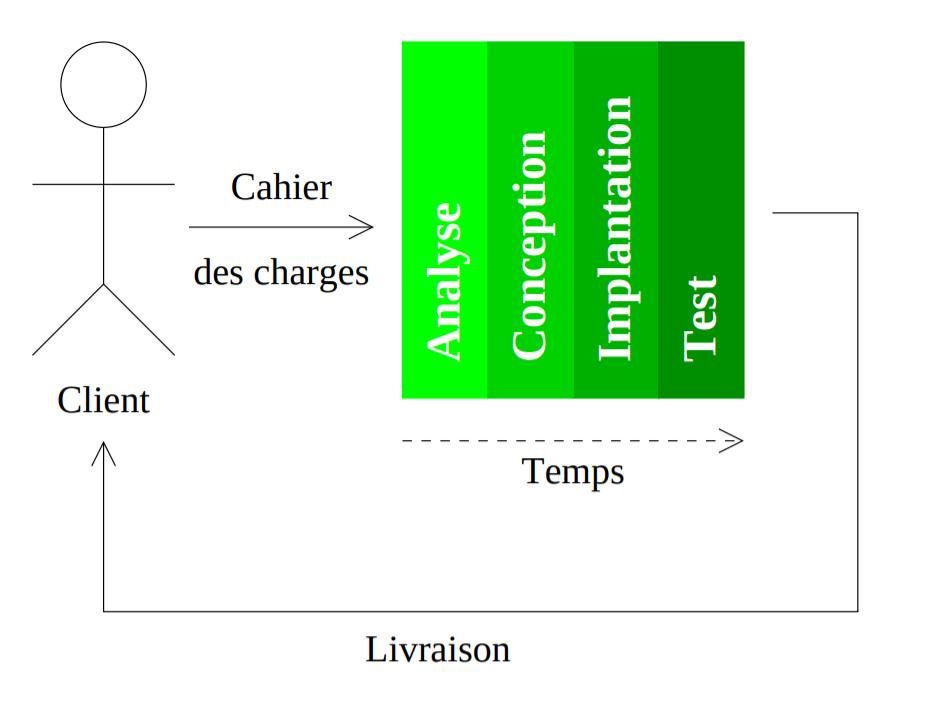
\includegraphics[width = 5in, height = 2.7in]{../Images/Analyse_Conception.png}
\caption{Développement en cascade}
\end{figure}

\newpage

\section{Méthodes utilisée}

\subsection{UML}
Le langage de modélisation unifié (UML) est un langage de modélisation de développement à usage général dans le domaine du génie logiciel qui vise à fournir un moyen standard de visualiser la conception d'un système.
\\\\
La création d'UML était à l'origine motivée par le désir de standardiser les systèmes de notation disparates et les approches de conception de logiciels. Il a été développé par Grady Booch, Ivar Jacobson et James Rumbaugh chez Rational Software en 1994–1995, avec un développement ultérieur dirigé par eux jusqu'en 1996.

\begin{figure}[h]
\centering
    
\includegraphics[width = 4in, height = 2in]{../Images/UMLlogo.png}
\caption{Unified Modeling Language}
\end{figure}

\vspace{-0.1in}
\subsection{PlantUML}
PlantUML est un outil open source permettant aux utilisateurs de cr\'eer des diagrammes UML \`a partir d'un langage de texte brut. Le langage de PlantUML est un exemple de langage sp\'ecifique au domaine. Il utilise le logiciel Graphviz pour disposer ses diagrammes. Il a \'et\'e utilis\'e pour permettre aux \'etudiants aveugles de travailler avec UML\@. PlantUML aide \'egalement les ing\'enieurs logiciels aveugles \`a concevoir et lire des diagrammes UML\@.

\vspace{-0.2in}

\begin{figure}[h]
\centering
    
\includegraphics[width = 3.6in, height = 1.9in]{../Images/plantuml.png}
\vspace{-0.1in}
\caption{PlantUML}
\end{figure}

\newpage

\subsection{PlantUML Previewer}
Plantuml previewer est un plugin (App) pour Vim qui permet d'afficher un code écrit en Vim et essentiellement de compiler et d'exécuter ce code instantanément dans un navigateur choisi (Chrome, Safari, Firefox...) notez que cela devrait avoir le `open-browser.vim  plugin' installé pour ouvrir le navigateur par défaut et a plus de dépendances comme Graphviz et JAVA et sûrement assez Vim.
\\
Vous pouvez trouver la description de ces programmes ci-dessous :

\vspace{0.05in}

\begin{figure}[h]
\centering
    \fbox{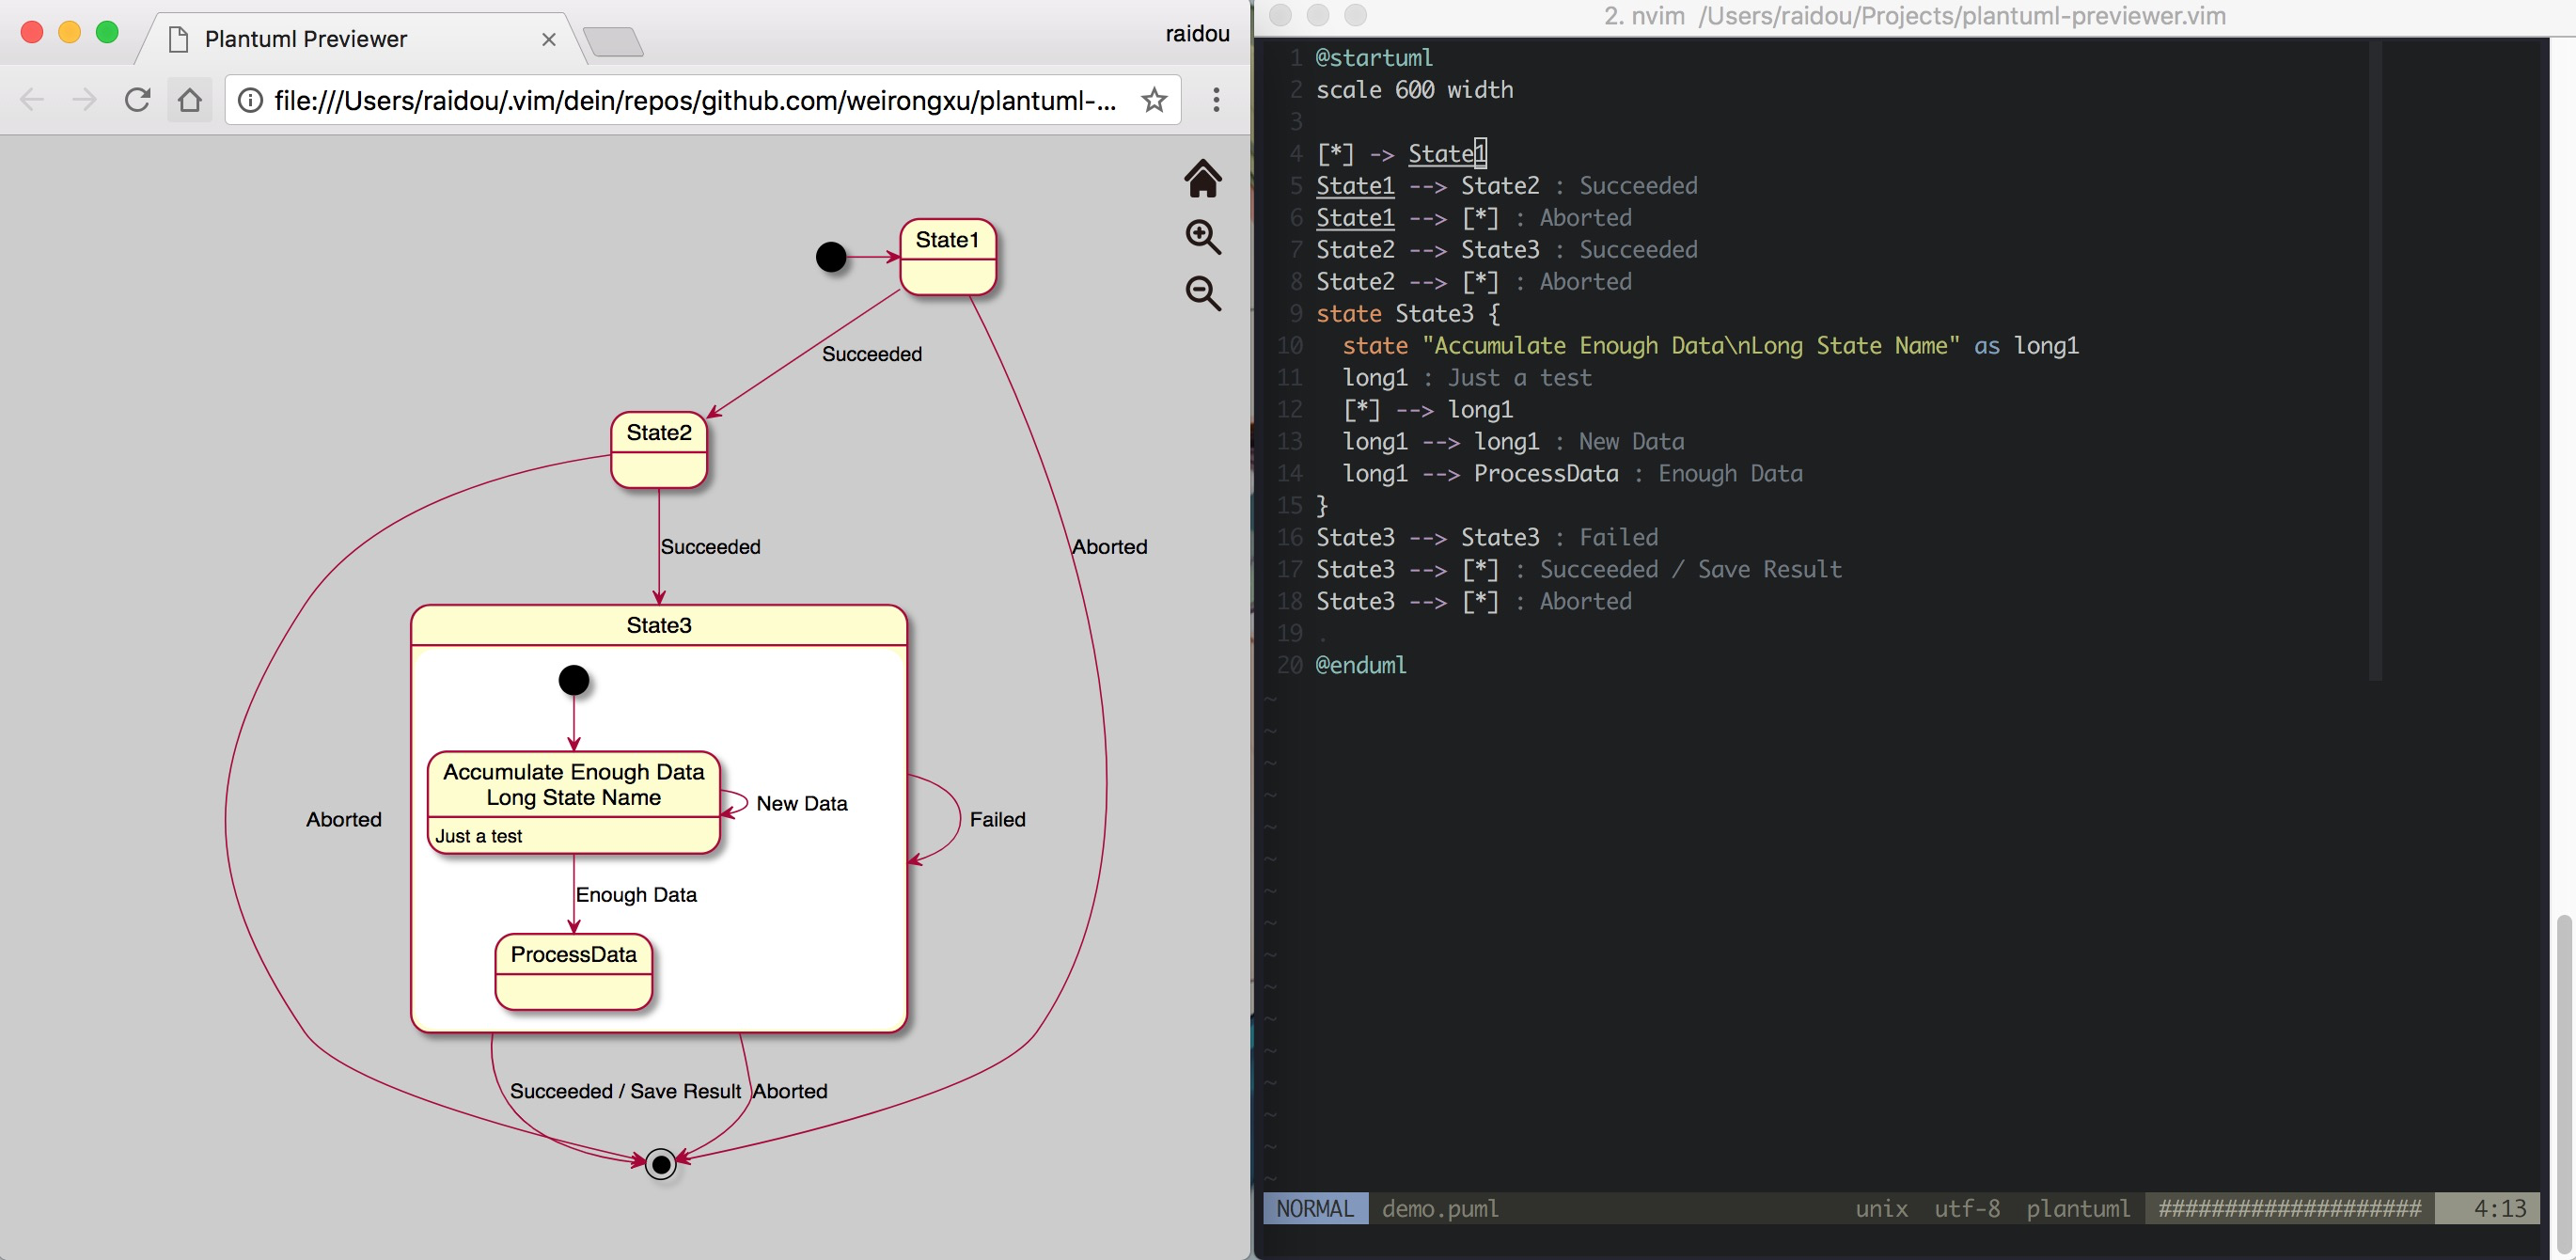
\includegraphics[width = 6.6in, height = 3in]{../Images/PlantumlPreviewer.png}}
    \caption{PlantUML preview example}
\end{figure}

\vspace{-0.2in}
\subsection{Graphviz}
Graphviz est un logiciel de visualisation graphique open source. La visualisation de graphes est un moyen de représenter des informations structurelles sous forme de diagrammes de graphes et de réseaux abstraits. Il a des applications importantes dans les réseaux, la bio-informatique, le génie logiciel, la conception de bases de données et de sites Web, l'apprentissage automatique et les interfaces visuelles pour d'autres domaines techniques.

\begin{figure}[h]
\centering
    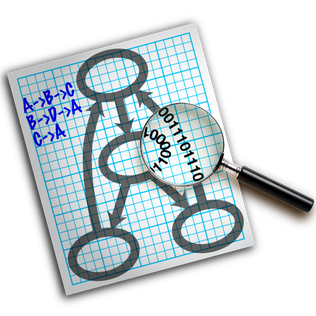
\includegraphics[width = 4in, height = 2in]{../Images/GraphvizLogo.png}
    \caption{Graphviz logo}
\end{figure}

\newpage

\subsection{Vim}
Vim est le programme le plus important (une contraction de Vi IMproved) est un clone, avec des ajouts, Il est conçu pour être utilisé à la fois à partir d'une interface de ligne de commande (TUI) et en tant qu'application autonome dans une interface utilisateur graphique. Vim est un logiciel gratuit et open-source et est publié sous une licence qui inclut des clauses de charityware, encourageant les utilisateurs qui apprécient le logiciel à envisager de faire un don à des enfants en Ouganda. La licence est compatible avec la Licence Publique Générale GNU grâce à une clause spéciale permettant la distribution de copies modifiées "sous la version 2 de GNU GPL ou toute version ultérieure".

\vspace{0.2in}

\begin{figure}[h]
\centering
    
\includegraphics[width = 3.5in, height = 2in]{../Images/Vim.png}
    \caption{Visual Editor iMproved (text editor)}
\end{figure}

\section{Diagrammes}

\subsection{Diagrammes de cas d'utilisation}

Un diagramme de cas d'utilisation dans sa forme la plus simple est une représentation de l'interaction d'un utilisateur avec le système qui montre la relation entre l'utilisateur et les différents cas d'utilisation dans lesquels l'utilisateur est impliqué. Un diagramme de cas d'utilisation peut identifier les différents types d'utilisateurs d'un système et les différents cas d'utilisation et seront souvent accompagnés également d'autres types de diagrammes.

\vspace{0.2in}

\begin{figure}[h]
\centering
    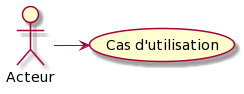
\includegraphics[width = 3.0in, height = 1.0in]{../Images/usecaseEG.png}
    \caption{Exemple de cas d'utilisation}
\end{figure}

\newpage

\subsubsection{Identification des acteurs}
\begin{itemize}
\item Utilisateur : peut être un étudiant, un enseignant, un administrateur ou simplement un visiteur.
\item Administrateur : c'est lui qui va gérer les étudiants et les enseignants (Ajouter, Modifier et Supprimer).
\item Étudiant : il va gérer ses recours (l'ajout, la modification et la suppression).
\item Enseignant : il va gérer les recours soumis (refuser ou valider)
\end{itemize}

\subsubsection{Identification des cas d'utilisation et description textuelle}

\begin{table}[h]
\centering
\begin{tabular}{|l|l|l|}
\hline
\rowcolor[HTML]{9B9B9B}
\textbf{Cas d'utilisation} & \textbf{Acteur} & \textbf{Message}                                                                                                        \\ \hline
\rowcolor[HTML]{DAE8FC}
S'authentifier             & Utilisateur     & \begin{tabular}[c]{@{}l@{}}Émet : Username / Password\\ Reçoit : Droit d'accès\end{tabular}                               \\ \hline
\rowcolor[HTML]{ECF4FF}
Gestion des recours        & Étudiant        & \begin{tabular}[c]{@{}l@{}}Émet : (Ajouter, Modifier, Supprimer,\\ Consulter)\\ Reçoit : Opération effectuer\end{tabular} \\ \hline
\rowcolor[HTML]{DAE8FC}
Gestion des étudiants      & Administrateur  & \begin{tabular}[c]{@{}l@{}}Émet : (Ajouter, Modifier, Supprimer,Valider)\\ Reçoit : Opération effectuer\end{tabular}      \\ \hline
\rowcolor[HTML]{ECF4FF}
Gestion des enseignants    & Administrateur  & \begin{tabular}[c]{@{}l@{}}Émet : (Ajouter, Modifier, Supprimer,Valider)\\ Reçoit : Opération effectuer\end{tabular}      \\ \hline
\rowcolor[HTML]{DAE8FC}
Valider recours            & Enseignant      & \begin{tabular}[c]{@{}l@{}}Émet : Clique bouton\\ Reçoit : Recours valider.\end{tabular}                                  \\ \hline
\rowcolor[HTML]{ECF4FF}
Refuser recours            & Enseignant      & \begin{tabular}[c]{@{}l@{}}Émet : Clique bouton\\ Reçoit : Recours refuser.\end{tabular}                                  \\ \hline
\end{tabular}
    \caption{Les acteurs, leurs cas d'utilisation avec les messages(Émet, Reçu).}
\end{table}

\vspace{-0.3in}

\subsubsection{\large{Les diagrammes de cas d'utilisation avec descriptions}}

\vspace{-0.1in}

\begin{figure}[h]
\centering
  \vspace{-0.1in}
    \centerline{\fbox{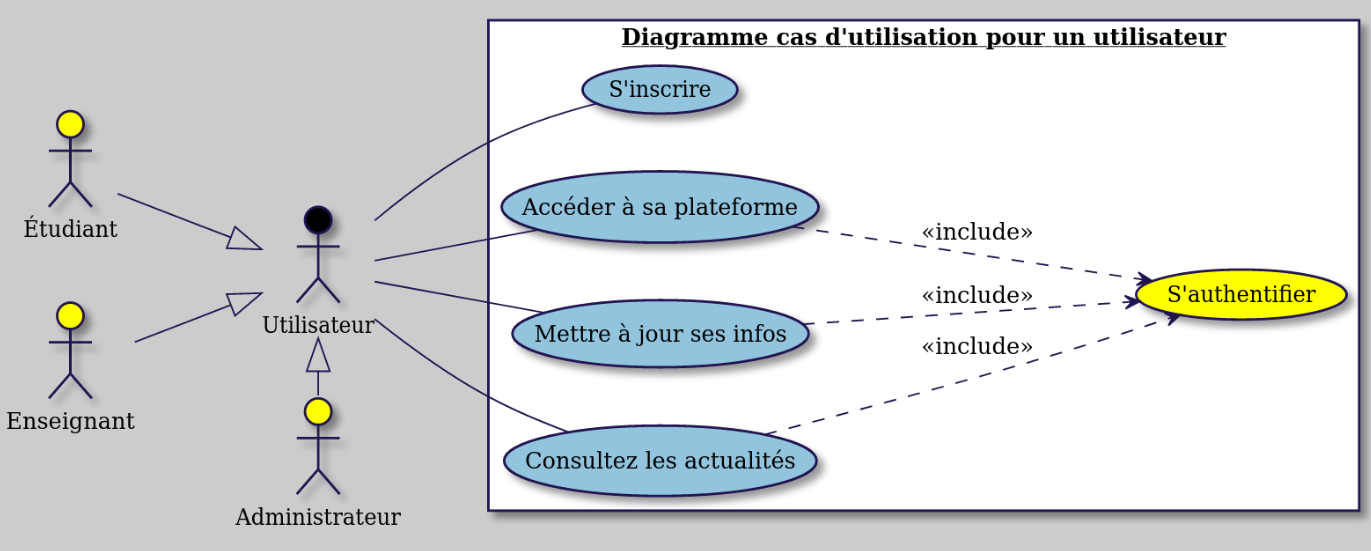
\includegraphics[width = 6.6in, height = 3.1in]{../Conception/Usecase/PNG/General/Utilisateur3.png}}}
    \caption{Diagramme de cas d'utilisation pour un Utilisateur}
\end{figure}

\newpage

\begin{figure}[h]
\centering
    \centerline{\fbox{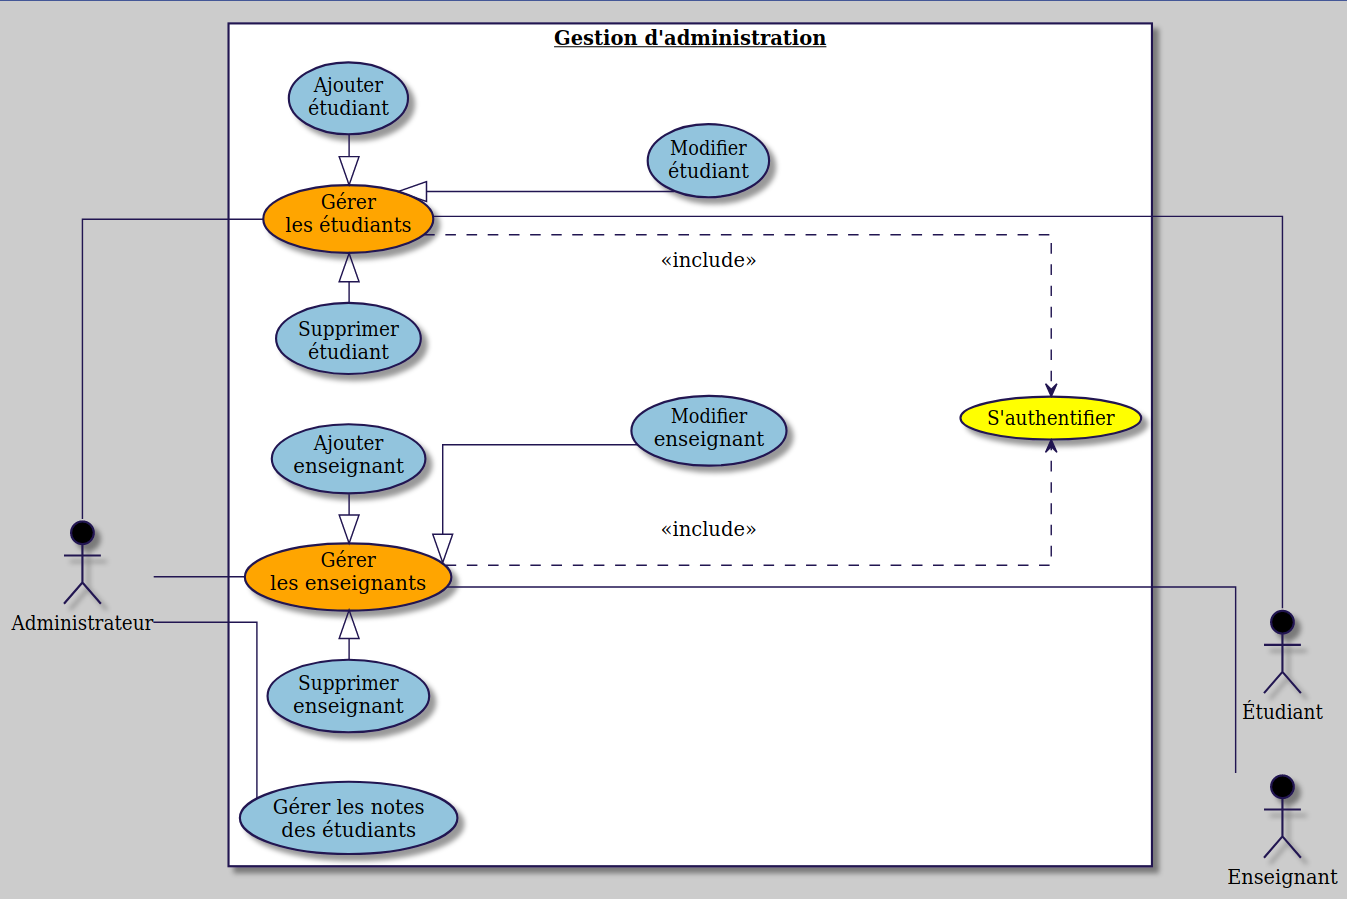
\includegraphics[width = 6.6in, height = 6in]{../Conception/Usecase/PNG/Administrateur.png}}}
    \caption{Diagramme de cas d'utilisation pour l'administrateur}
\end{figure}

\textbf{Description :}

\begin{itemize}
    \item L'administrateur peut gérer les étudiants et les enseignants en:
\begin{itemize}
    \item ajoutant leurs informations.
    \item modifiant leurs informations.
    \item supprimant leurs informations.
\end{itemize}
    \item L'administrateur doit d'abord s'authentifier.
    \item L'administrateur peut gérer les notes des étudiants.
\end{itemize}

\newpage

\textbf{Cas d'utilisation détaillée :}

\begin{figure}[h]
\centering
    \centerline{\fbox{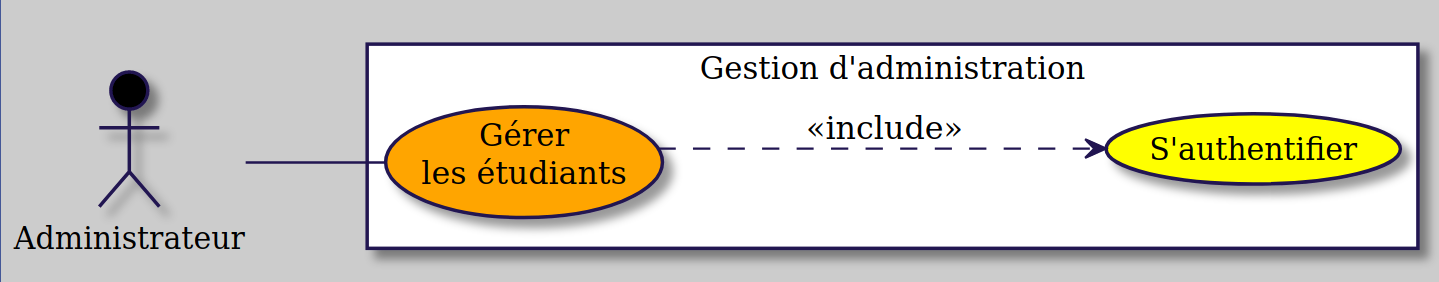
\includegraphics[width = 6in, height = 1in]{../Conception/Usecase/PNG/Details/GererET.png}}}
    \caption{Cas d'utilisation <<Gérer les étudiants>>}
\end{figure}

\vspace{-0.1in}

\begin{table}[h]
\centering
\begin{tabular}{|c|l|}
\hline
\rowcolor[HTML]{ECF4FF} 
\textbf{Nom de cas d'utilisation}  & Gérer les étudiants.                                                                                                                                                                                                                                                                                                                                                                                                                                                                                                            \\ \hline
\rowcolor[HTML]{DAE8FC} 
\textbf{Acteur Principale}         & Administration                                                                                                                                                                                                                                                                                                                                                                                                                                                                                                                  \\ \hline
\rowcolor[HTML]{ECF4FF} 
\textbf{Acteur Secondaire}         & Étudiant                                                                                                                                                                                                                                                                                                                                                                                                                                                                                                                        \\ \hline
\rowcolor[HTML]{DAE8FC} 
\textbf{Objectif}                  & \begin{tabular}[c]{@{}l@{}}Donner à l'administration la possibilité d’ajouter des étudiants,\\ supprimer ou modifier un étudiant qui existe déjà.\end{tabular}                                                                                                                                                                                                                                                                                                                                                                  \\ \hline
\rowcolor[HTML]{ECF4FF} 
\textbf{Pré condition}             & Authentification.                                                                                                                                                                                                                                                                                                                                                                                                                                                                                                               \\ \hline
\rowcolor[HTML]{DAE8FC} 
\textbf{Séquencement nominal}      & \begin{tabular}[c]{@{}l@{}}1.Lancer l’application Web.\\ 2.Le site affiche la page de la connexion.\\ 3.Choisissez le type de traitement de l’étudiant.\\ 4.Traiter l’opération choisie.\\ 5.Message de validation.\end{tabular}                                                                                                                                                                                                                                                                                                \\ \hline
\rowcolor[HTML]{ECF4FF} 
\textbf{Séquencement alternatif}   & \begin{tabular}[c]{@{}l@{}}A1.Si le choix est ajouter :\\   A1.1. Remplir les informations de l'étudiant (nom, prénom...).\\   A1.2. Le système vérifie la validation des informations fournis.\\ A2. Si le choix est modifier :\\   A2.1. L’administrateur choisissez l’enseignant à modifie.\\   A2.2. Remplissez les champs à modifier.\\ A3. Si le choix est supprimer :\\   A3.1. L’administrateur choisissez l’enseignant à supprimer.\\   A3.2. Confirmer la suppression de l’enseignant.\end{tabular} \\ \hline
\rowcolor[HTML]{DAE8FC} 
\textbf{Séquencement exceptionnel} & \begin{tabular}[c]{@{}l@{}}Si les informations de l’étudiant ne sont pas correctes,\\ nous générons un message d'erreur. (4).\end{tabular}                                                                                                                                                                                                                                                                                                                                                                                       \\ \hline
\end{tabular}
    \caption{Fiche descriptive <<Gérer les étudiants>>}
\end{table}

\begin{figure}[H]
\centering
  \vspace{-0.1in}
    \centerline{\fbox{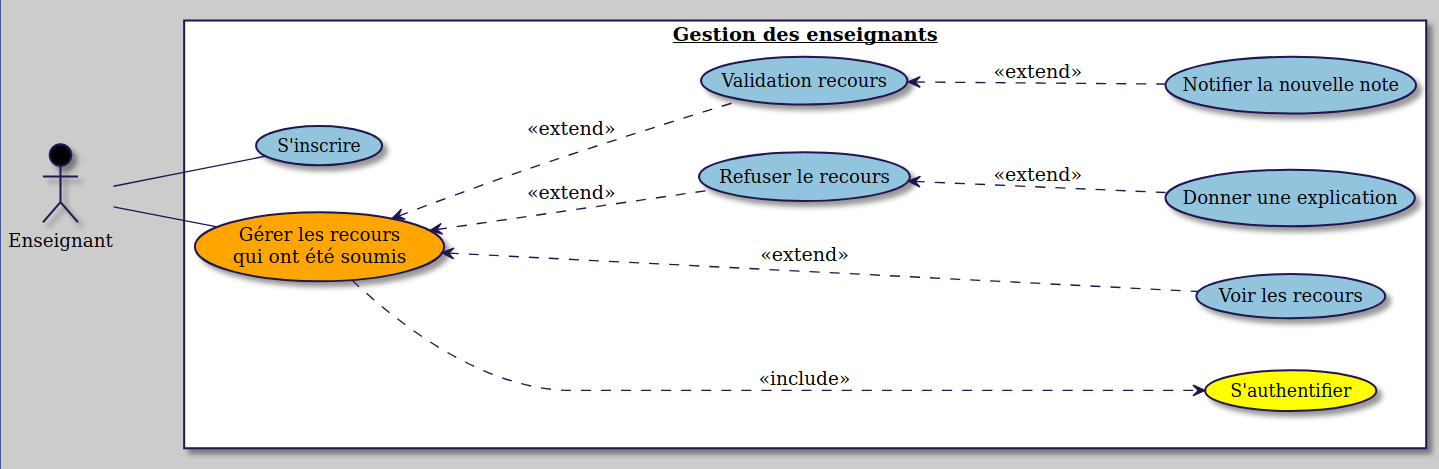
\includegraphics[width = 6.6in, height = 3in]{../Conception/Usecase/PNG/Enseignant.png}}}
    \caption{Diagramme de cas d'utilisation pour l'enseignant}
  \vspace*{-0.3in}
\end{figure}

\newpage

\vspace{0.1in}

\textbf{Description :}

\begin{itemize}
    \item L'enseignant peut s'inscrire.
    \item L'enseignant choisira l'une des options ci-dessous :
    \begin{itemize}
        \item Valider le recours.
        \item Refuser le recours.
    \end{itemize}
    \item L'enseignant doit s'authentifier pour gérer les recours qui ont été soumis.
\end{itemize}

\vspace{0.2in}

\textbf{Cas d'utilisation détaillée :}

\vspace{0.2in}

\begin{figure}[h]
\centering
    \centerline{\fbox{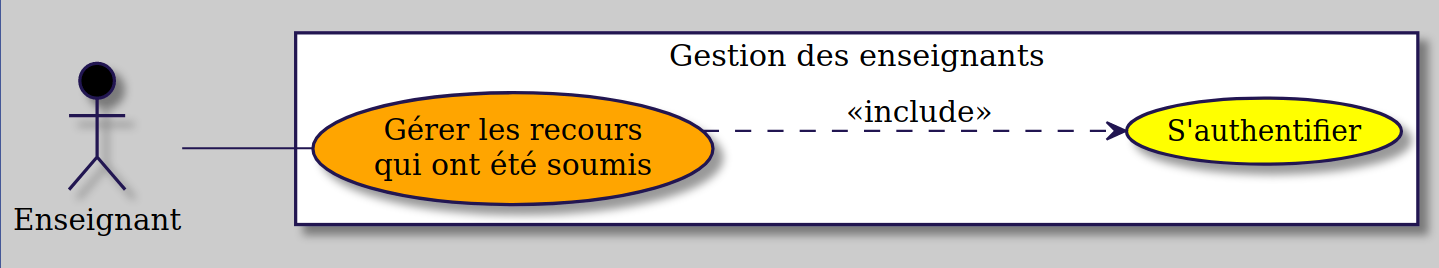
\includegraphics[width = 6in, height = 1in]{../Conception/Usecase/PNG/Details/GererRecoursSoumis.png}}}
    \caption{Cas d'utilisation <<Gérer les recours qui on été soumis>>}
\end{figure}

\begin{table}[h]
\centering
\begin{tabular}{|c|l|}
\hline
\rowcolor[HTML]{ECF4FF}
\textbf{Nom de cas d'utilisation}  & Gérer les recours qui ont été soumis                                                                                                                                                                                                                                                                                  \\ \hline
\rowcolor[HTML]{DAE8FC}
\textbf{Acteur Principale}         & Enseignant                                                                                                                                                                                                                                                                                                            \\ \hline
\rowcolor[HTML]{ECF4FF}
\textbf{Acteur Secondaire}         & Interface Web, Base de données                                                                                                                                                                                                                                                                                        \\ \hline
\rowcolor[HTML]{DAE8FC}
\textbf{Objectif}                  & \begin{tabular}[c]{@{}l@{}}Rendre disponibles pour un enseignant d'autoriser ou refuser un\\ recours soumis par un étudiant avec des options supplémentaires.\end{tabular}                                                                                                                                            \\ \hline
\rowcolor[HTML]{ECF4FF}
\textbf{Pré condition}             & Authentification                                                                                                                                                                                                                                                                                                      \\ \hline
\rowcolor[HTML]{DAE8FC}
\textbf{Séquencement nominal}      & \begin{tabular}[c]{@{}l@{}}n1. Lancer l’application Web et s’authentifier en tant\\ qu’enseignant.\\ n2. Choisissez un recours à traiter.\\ n3. Traiter le recours en acceptant ou refusant et avec des\\ informations supplémentaires sur le recours.\\ n4. Retourne aux page d’accueil.\end{tabular}                    \\ \hline
\rowcolor[HTML]{ECF4FF}
\textbf{Séquencement alternatif}   & \begin{tabular}[c]{@{}l@{}}a1. Si l’enseignant a accepté le recours, il peut choisir de notifier\\ l'étudiant de la nouvelle note ou non. Retourne au (n4).\\ a2. Si l’enseignant a refusé le recours, il peut ajouter une\\ explication sur le recours à l'étudiant ou non. Retourne au (n4).\end{tabular} \\ \hline
\rowcolor[HTML]{DAE8FC}
\textbf{Séquencement exceptionnel} & \begin{tabular}[c]{@{}l@{}}En cas ou la connexion ou le serveur n’est pas disponible on\\ actualise la page et retourne l’enseignant à la page d’accueil.\end{tabular}                                                                                                                                                \\ \hline
\rowcolor[HTML]{ECF4FF}
\textbf{Post condition}            & \begin{tabular}[c]{@{}l@{}}- Notifier l'étudiant de l'état de son recours.\\ - Sauvegarder les changements et toutes les actions entreprises\\ dans un fichier log pour être vu par l’administration.\end{tabular}                                                                                                    \\ \hline
\end{tabular}
    \caption{Fiche descriptive <<Gérer les recours qui on été soumis>>}
\end{table}

\newpage

\begin{figure}[h]
\centering
    \centerline{\fbox{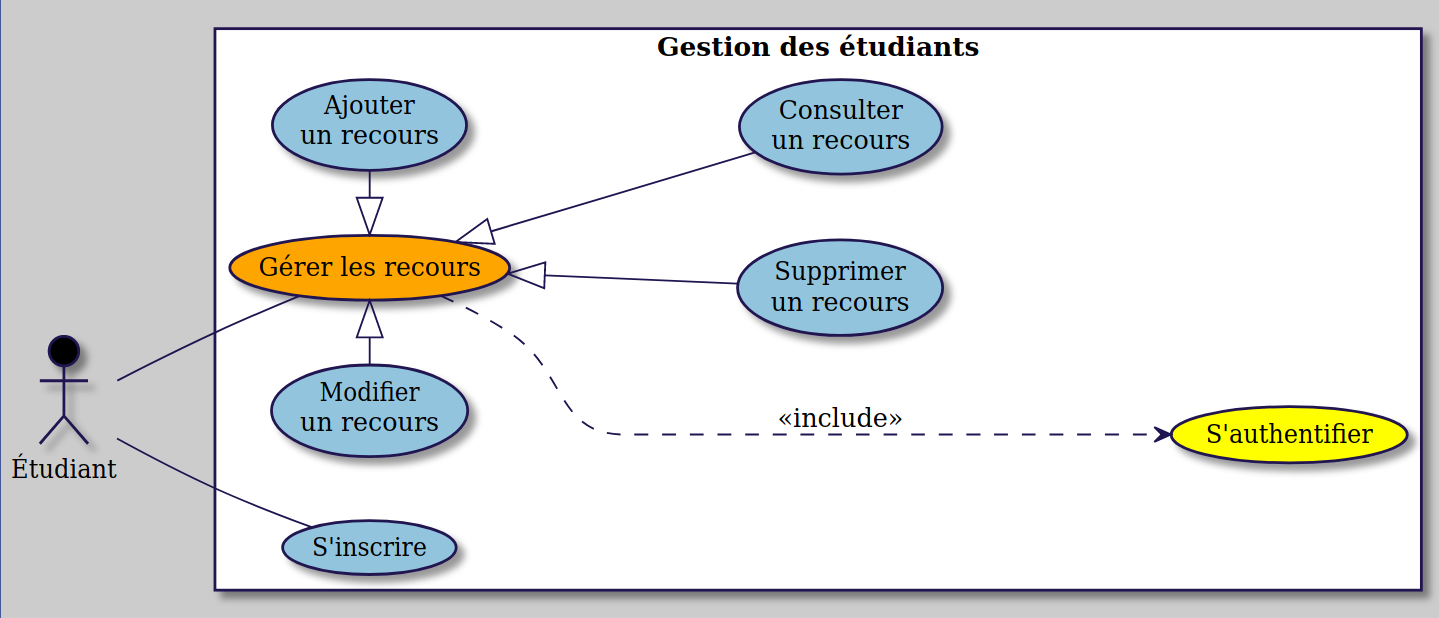
\includegraphics[width = 6.6in, height = 3in]{../Conception/Usecase/PNG/Etudiant.png}}}
    \caption{Diagramme de cas d'utilisation pour l'étudiant}
\end{figure}

\vspace{-0.15in}

\textbf{Description :}

\begin{itemize}
    \item L'étudiant peut s'inscrire.
    \item L'étudiant choisira d'ajouter, modifier, supprimer ou consulter un recours après l’authentifié.
\end{itemize}

\textbf{Cas d'utilisation détaillée :}

\vspace*{0.1in}

\begin{figure}[h]
\centering
    \centerline{\fbox{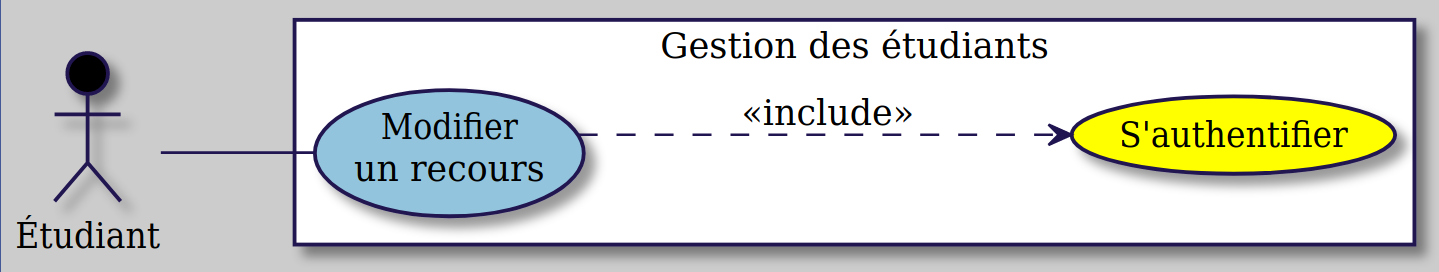
\includegraphics[width = 6in, height = 1in]{../Conception/Usecase/PNG/Details/ModifierRecours.png}}}
    \caption{Cas d'utilisation <<Modifier un recours>>}
\end{figure}

\vspace*{-0.1in}

\begin{table}[h]
  \vspace*{-0.01in}
\centering
\begin{tabular}{|c|l|}
\hline
\rowcolor[HTML]{ECF4FF}
\textbf{Nom de cas d'utilisation}  & Modifier un recours                                                                                                                                                                                                                                   \\ \hline
\rowcolor[HTML]{DAE8FC}
\textbf{Acteur Principale}         & Étudiant                                                                                                                                                                                                                                              \\ \hline
\rowcolor[HTML]{ECF4FF}
\textbf{Acteur Secondaire}         & Site Web                                                                                                                                                                                                                                              \\ \hline
\rowcolor[HTML]{DAE8FC}
\textbf{Objectif}                  & \begin{tabular}[c]{@{}l@{}}Permet l'étudiant de modifier un recours déjà soumis.\end{tabular}                                                                                                                                                       \\ \hline
\rowcolor[HTML]{ECF4FF}
\textbf{Pré condition}             & Authentification                                                                                                                                                                                                                                      \\ \hline
\rowcolor[HTML]{DAE8FC}
\textbf{Séquencement nominal}      & \begin{tabular}[c]{@{}l@{}}1. Lancer l’application Web et s’authentifier en tant qu’étudiant.\\ 2. Choisissez le recours qu'il souhaite modifier.\\ 3. Remplissez les champs à  modifier.\\ 4. Soumettez la modification.\end{tabular} \\ \hline
\rowcolor[HTML]{ECF4FF}
\textbf{Séquencement alternatif}   & \begin{tabular}[c]{@{}l@{}}Si les informations ne correspondent pas à l'étudiant, nous\\ générons un message d'erreur.\end{tabular}                                                                                                              \\ \hline
\rowcolor[HTML]{DAE8FC}
\textbf{Séquencement exceptionnel} & \begin{tabular}[c]{@{}l@{}}- En cas ou la connexion ou le serveur n’est pas disponible on\\ actualise la page et retourne l’étudiant à la page d’accueil.\end{tabular}                                                                             \\ \hline
\rowcolor[HTML]{ECF4FF}
\textbf{Post condition}            & \begin{tabular}[c]{@{}l@{}}- Assurer la livraison du nouveau recours aux enseignant.\\ - Informer l’étudiant que le recours à été modifié avec succès.\end{tabular}                                                         \\ \hline
\end{tabular}
    \caption{Fiche descriptive <<Modifier un recours>>}
  \vspace*{-0.7in}
\end{table}

\newpage

\begin{figure}[h]
\centering
    \centerline{\fbox{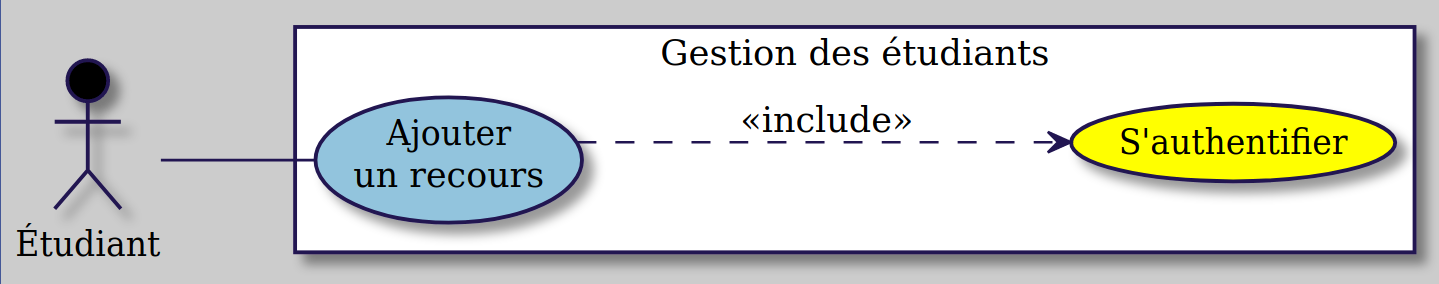
\includegraphics[width = 6in, height = 1in]{../Conception/Usecase/PNG/Details/AjouterRecours.png}}}
    \caption{Cas d'utilisation <<Ajouter un recours>>}
\end{figure}

\vspace*{-0.1in}

\begin{table}[h]
\centering
\begin{tabular}{|c|l|}
\hline
\rowcolor[HTML]{ECF4FF}
\textbf{Nom de cas d'utilisation}  & Ajouter un recours                                                                                                                                                                                                                                                                                                                                                                                                                                                \\ \hline
\rowcolor[HTML]{DAE8FC}
\textbf{Acteur Principale}         & Étudiant                                                                                                                                                                                                                                                                                                                                                                                                                                                          \\ \hline
\rowcolor[HTML]{ECF4FF}
\textbf{Acteur Secondaire}         & Site Web                                                                                                                                                                                                                                                                                                                                                                                                                                                          \\ \hline
\rowcolor[HTML]{DAE8FC}
\textbf{Objectif}                  & \begin{tabular}[c]{@{}l@{}}Donner à l'étudiant la possibilité d'ajouter un recours avec\\ ses informations (module, enseignant, description,...).\end{tabular}                                                                                                                                                                                                                                                                          \\ \hline
\rowcolor[HTML]{ECF4FF}
\textbf{Pré condition}             & Authentification                                                                                                                                                                                                                                                                                                                                                                                                                                                  \\ \hline
\rowcolor[HTML]{DAE8FC}
\textbf{Séquencement nominal}      & \begin{tabular}[c]{@{}l@{}}1. Lancer l’application Web et s’authentifier en tant qu’étudiant.\\ 2. Remplir les informations (nom, prénom, matricule,...).\\ 3. Choisissez le module et la filière.\\ 4. Ajouter une explication (commentaire) sur l'endroit où le\\ défaut pourrait être (nombre d'exercice ou question...).\\ 5. Ajoutez une photo pour une description détaillée (facultative).\\ 6. Soumettre le recours.\end{tabular}   \\ \hline
\rowcolor[HTML]{ECF4FF}
    \textbf{Séquencement alternatif}   & \begin{tabular}[c]{@{}l@{}}A1. Si les informations ne correspondent pas à l'étudiant, nous\\ générons un message d'erreur.\end{tabular}                                                                                                                                                                                                                                                                                                                           \\ \hline
\rowcolor[HTML]{DAE8FC}
\textbf{Séquencement exceptionnel} & \begin{tabular}[c]{@{}l@{}}- En cas ou la connexion ou le serveur n’est pas disponible on\\ actualise la page et retourne l’étudiant à la page d’accueil.\end{tabular}                                                                                                                                                                                                                                                                                             \\ \hline
\rowcolor[HTML]{ECF4FF}
\textbf{Post condition}            & \begin{tabular}[c]{@{}l@{}}- Enregistrez plusieurs copies pour ne pas perdre le recours.\\ - Assurer la livraison du recours aux enseignant.\\ - Nous voulons nous assurer que l'étudiant est informé de la\\ livraison du recours.\end{tabular} \\ \hline
\end{tabular}
    \caption{Fiche descriptive <<Ajouter un recours>>}
  \vspace*{-0.2in}
\end{table}

\begin{figure}[H]
\centering
    \centerline{\fbox{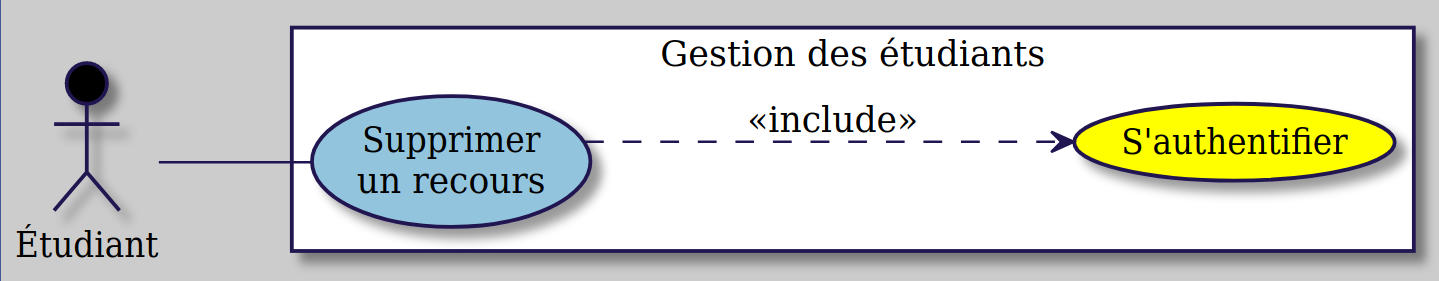
\includegraphics[width = 6in, height = 1in]{../Conception/Usecase/PNG/Details/SupprimerRecours.png}}}
    \vspace{-0.08in}
    \caption{Cas d'utilisation <<Supprimer un recours>>}
\end{figure}

\vspace{-0.15in}

\begin{table}[h]
\centering
\begin{tabular}{|c|l|}
\hline
\rowcolor[HTML]{ECF4FF} 
\textbf{Nom de cas d'utilisation}  & Supprimer un recours                                                                                                                                                                         \\ \hline
\rowcolor[HTML]{DAE8FC} 
\textbf{Acteur Principale}         & Étudiant                                                                                                                                                                                     \\ \hline
\rowcolor[HTML]{ECF4FF} 
\textbf{Acteur Secondaire}         & Site Web                                                                                                                                                                                     \\ \hline
\rowcolor[HTML]{DAE8FC} 
\textbf{Objectif}                  & Donnez à l'étudiant la possibilité de supprimer le recours.                                                                                                                                  \\ \hline
\rowcolor[HTML]{ECF4FF} 
\textbf{Pré condition}             & Authentification                                                                                                                                                                             \\ \hline
\rowcolor[HTML]{DAE8FC} 
\textbf{Séquencement nominal}      & \begin{tabular}[c]{@{}l@{}}1. Lancer l’application Web et s’authentifier en tant qu’étudiant.\\ 2. Choisissez le recours à supprimer.\\ 3. Confirmer la suppression du recours.\end{tabular} \\ \hline
\rowcolor[HTML]{DAE8FC} 
\textbf{Séquencement exceptionnel} & \begin{tabular}[c]{@{}l@{}}- En cas ou la connexion ou le serveur n’est pas disponible on\\ actualise la page et retourne l’étudiant a la page d’accueil.\end{tabular}                       \\ \hline
\rowcolor[HTML]{ECF4FF} 
\textbf{Post condition}            & - Informer l'étudiant que le recours a bien été supprimé.                                                                                                                                    \\ \hline
\end{tabular}
    \caption{Fiche descriptive <<Supprimer un recours>>}
  \vspace*{-2in}
\end{table}

\newpage

\begin{figure}[h]
\centering
    \centerline{\fbox{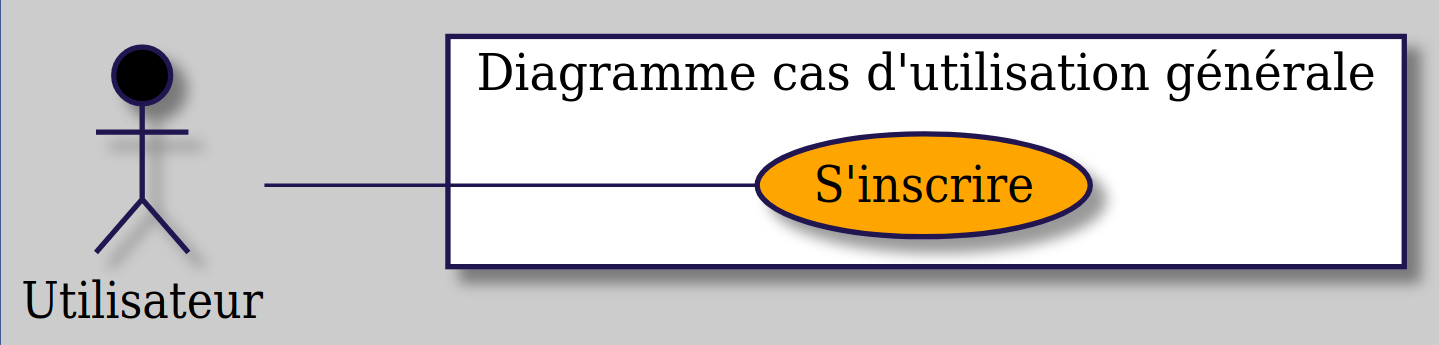
\includegraphics[width = 6in, height = 1in]{../Conception/Usecase/PNG/Details/S'inscrire.png}}}
    \vspace{-0.08in}
    \caption{Cas d'utilisation <<S'inscrire>>}
\end{figure}

\vspace*{-0.1in}

\begin{table}[h]
\centering
\begin{tabular}{|c|l|}
\hline
\rowcolor[HTML]{ECF4FF}
\textbf{Nom de cas d'utilisation}  & S'inscrire                                                                                                                                                                                                                    \\ \hline
\rowcolor[HTML]{DAE8FC}
\textbf{Acteur Principale}         & Étudiant, Enseignant                                                                                                                                                                                                          \\ \hline
\rowcolor[HTML]{ECF4FF}
\textbf{Acteur Secondaire}         & Site Web                                                                                                                                                                                                                      \\ \hline
\rowcolor[HTML]{DAE8FC}
\textbf{Objectif}                  & Permettre à l'étudiant ou au enseignant de s'inscrire.                                                                                                                                                                        \\ \hline
\rowcolor[HTML]{ECF4FF}
\textbf{Pré condition}             & Connexion internet                                                                                                                                                                                                            \\ \hline
\rowcolor[HTML]{DAE8FC}
\textbf{Séquencement nominal}      & \begin{tabular}[c]{@{}l@{}}1. Choisissez l'option d'inscription dans l'écran de ‘Login’.\\ 2. Remplir les informations (nom, prénom, matricule,...).\\ 3. Validez l'email par le code reçu dans la boite email.\end{tabular} \\ \hline
\rowcolor[HTML]{ECF4FF}
\textbf{Séquencement alternatif}   & \begin{tabular}[c]{@{}l@{}}A1. Validation du formulaire s'il y a des champs vides ou un\\ email invalide (doit être au format email '@ x.z') ou les mots\\ de passe ne correspondent pas.\end{tabular}                       \\ \hline
\rowcolor[HTML]{DAE8FC}
\textbf{Séquencement exceptionnel} & \begin{tabular}[c]{@{}l@{}}- En cas ou la connexion ou le serveur n’est pas disponible on\\ actualise la page ou affiche un erreur de connexion.\end{tabular}                                                                 \\ \hline
\end{tabular}
    \vspace{-0.05in}
    \caption{Fiche descriptive <<S'inscrire>>}
\end{table}

\vspace{-0.15in}

\subsection{Diagrammes de séquence}

Un diagramme de séquence montre les interactions d'objets organisées en séquence temporelle. Il décrit les objets et les classes impliqués dans le scénario et la séquence de messages échangés entre les objets nécessaires pour exécuter la fonctionnalité du scénario. Les diagrammes de séquence sont généralement associés aux réalisations de cas d'utilisation dans la vue logique du système en cours de développement. Les diagrammes de séquence sont parfois appelés diagrammes d'événements ou scénarios d'événements.

\vspace{0.2in}

\begin{figure}[h]
\centering
    \centerline{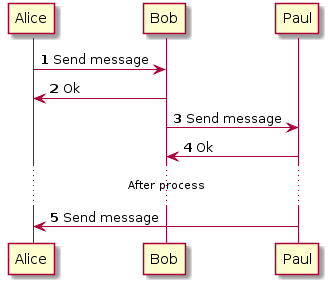
\includegraphics[width = 3.2in, height = 2.5in]{../Images/DiagSeqEX.png}}
    \caption{Exemple de diagramme de séquence}
\end{figure}

\newpage

\subsubsection{\large{Les diagrammes de séquences avec descriptions}}

\begin{figure}[h]
\centering
    \centerline{\fbox{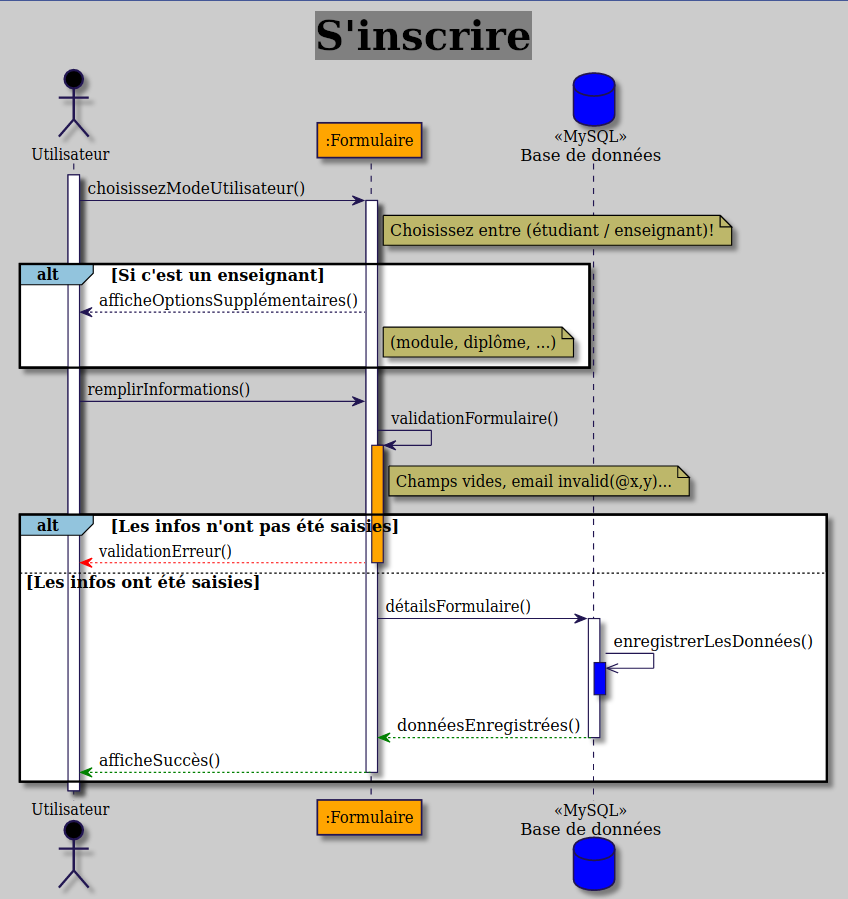
\includegraphics[width = 6.6in, height = 6.2in]{../Conception/Sequence/PNG/S'inscrire.png}}}
    \caption{Diagramme de séquences <<S'inscrire>>}
\end{figure}

\textbf{Description :}

\begin{itemize}
    \item Un utilisateur peut s'inscrire en tant que :
    \begin{itemize}
        \item Enseignant. (Diplôme, Module...)
        \item Étudiant.
    \end{itemize}
    \item Validation formulaire ``email sous la forme @x.y, Caractères spéciaux''
    \item Sauvegarde des données.
\end{itemize}

\newpage

\begin{figure}[h]
\centering
    \centerline{\fbox{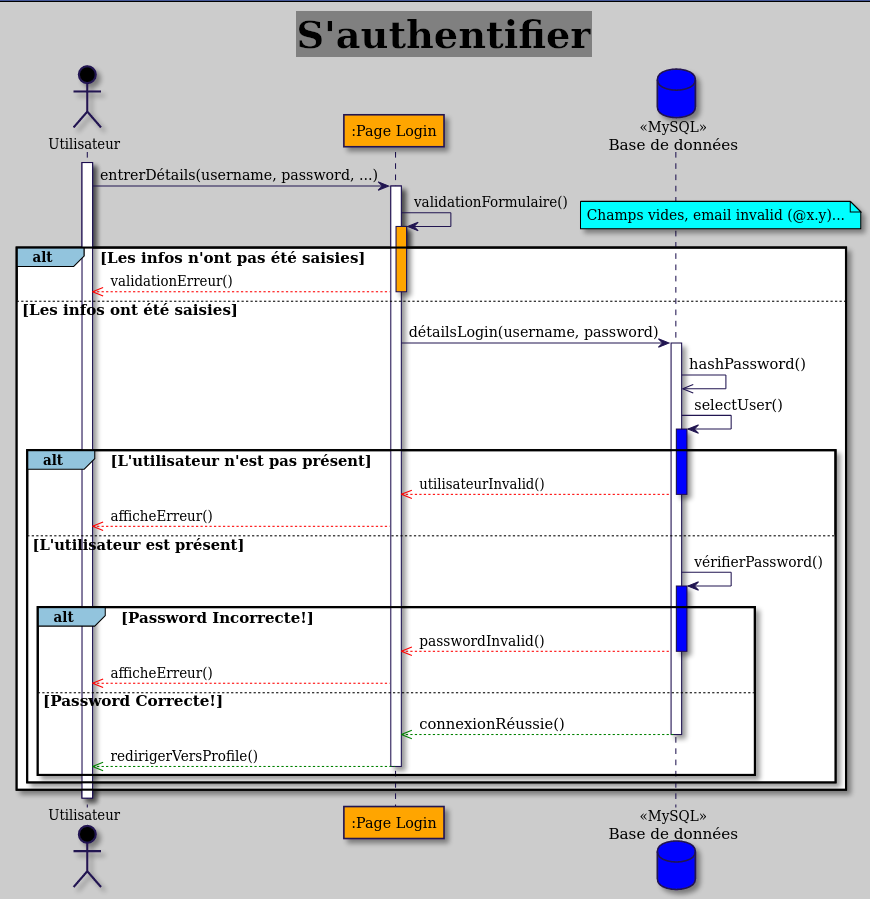
\includegraphics[width = 6.6in, height = 6.6in]{../Conception/Sequence/PNG/S'authentifier.png}}}
    \caption{Diagramme de séquences <<S'authentifier>>}
\end{figure}

\vspace{0.3in}

\textbf{Description :}

\begin{itemize}
    \item L'utilisateur saisira son nom d'utilisateur et son mot de passe.
    \item Le système vérifiera les informations données et générera des messages d'erreur s'il y en a autrement, il affichera un message de connexion réussie.
\end{itemize}

\newpage

\begin{figure}[h]
\centering
    \centerline{\fbox{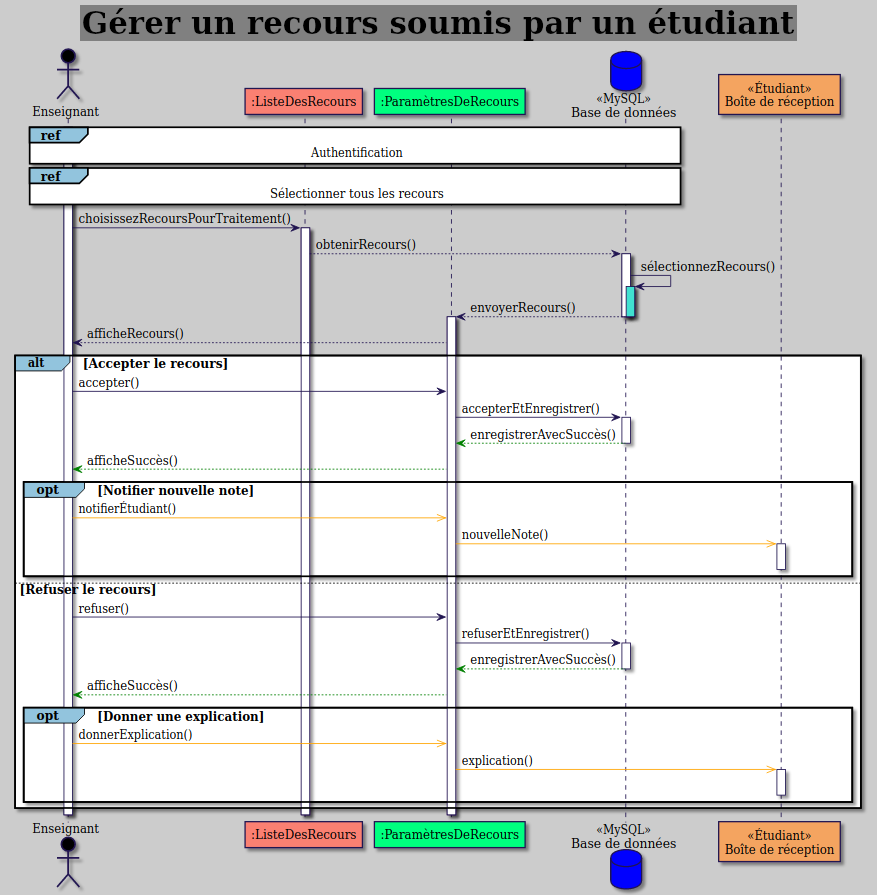
\includegraphics[width = 6.6in, height = 7.2in]{../Conception/Sequence/PNG/Enseignant/GererRecours.png}}}
    \caption{Diagramme de séquences <<Gérer un recours soumis par un étudiant>>}
\end{figure}

\textbf{Description :}

\begin{itemize}
    \item L'enseignant s'authentifiera d'abord puis le système générera une table des recours.
    \item L'enseignant validera ou refusera le recours et décidera de notifier l'étudiant ou non.
    \item La base de données <<MySQL>> enregistrera l'opération sous une forme d'une requête SQL
\end{itemize}

\newpage

\begin{figure}[h]
\centering
    \centerline{\fbox{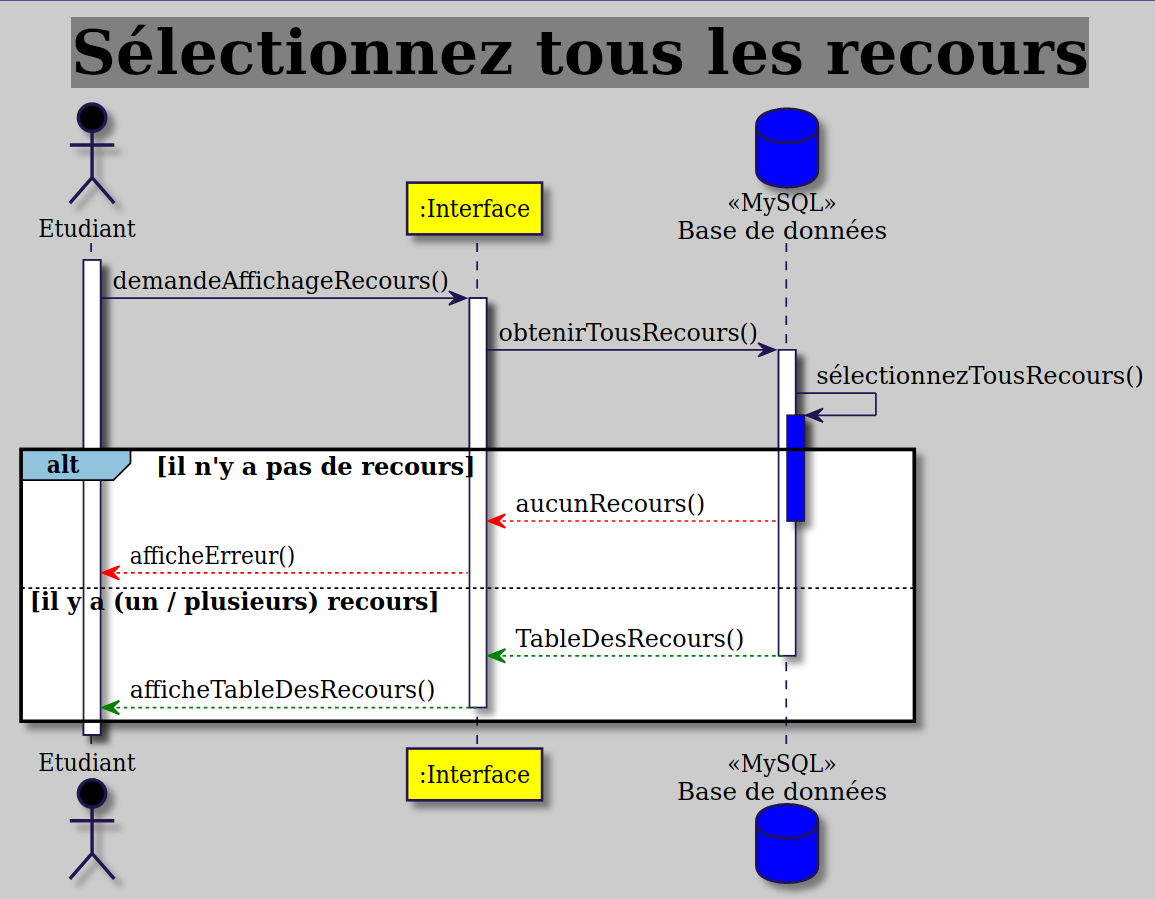
\includegraphics[width = 6.6in, height = 5.8in]{../Conception/Sequence/PNG/Etudiant/SelectTousRecours.png}}}
    \caption{Diagramme de séquences <<Sélectionnez tous les recours>>}
\end{figure}

\vspace{0.3in}

\textbf{Description :}

\begin{itemize}
    \item L'étudiant entrera dans la plate-forme où il pourra voir ses recours.
    \item Le système recherchera et sélectionnera tous les recours. 
    \item Si le système trouve des recours, le site Web générera un tableau contenant tous ses recours.
    \item Sinon, la page Web générera un message d'erreur (Aucun recours).
\end{itemize}

\newpage

\begin{figure}[h]
\centering
    \centerline{\fbox{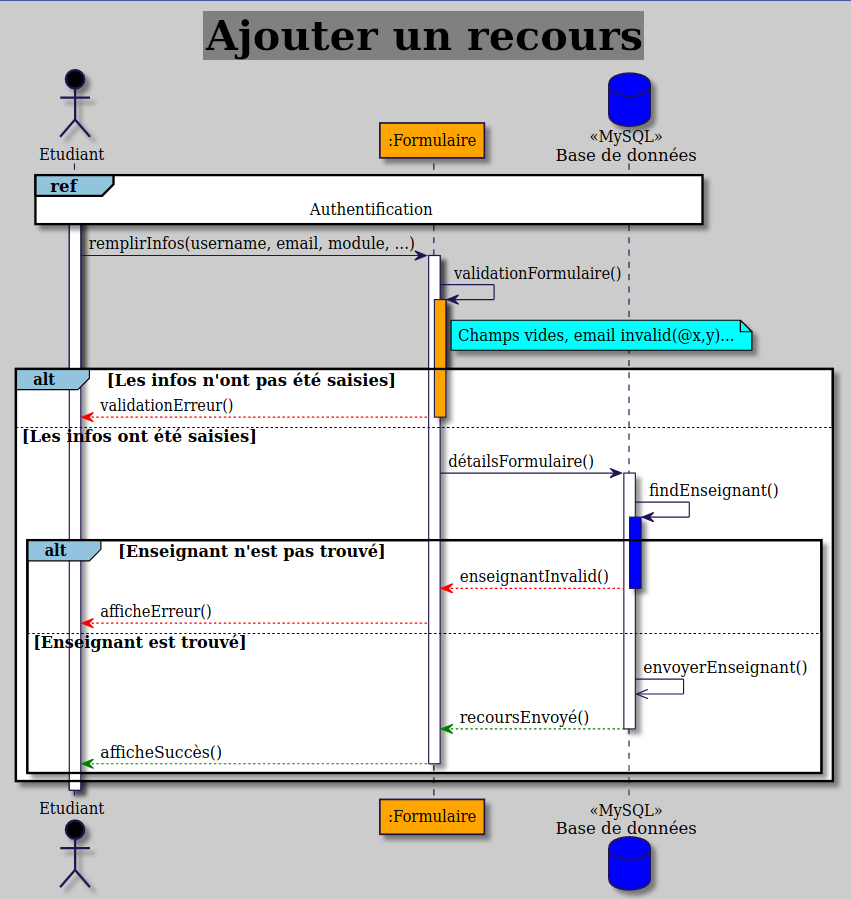
\includegraphics[width = 6.6in, height = 6.2in]{../Conception/Sequence/PNG/Etudiant/AjouterRecours.png}}}
    \caption{Diagramme de séquences <<Ajouter un recours>>}
\end{figure}

\textbf{Description :}

\begin{itemize}
    \item L'étudiant doit d'abord s'authentifier.
    \item Il remplit les informations de recours dans le formulaire affiché par le site Web.
    \item S'il y a des erreurs concernant des caractères spéciaux ou des champs vides, nous les afficherons. Sinon, le système recherchera l'enseignant concerné.
    \item Si l'enseignant est trouvé, le système lui enverra le recours et affichera un message de réussite à l'étudiant sinon, il affichera un message d'erreur.
\end{itemize}

\newpage

\begin{figure}[h]
\centering
    \centerline{\fbox{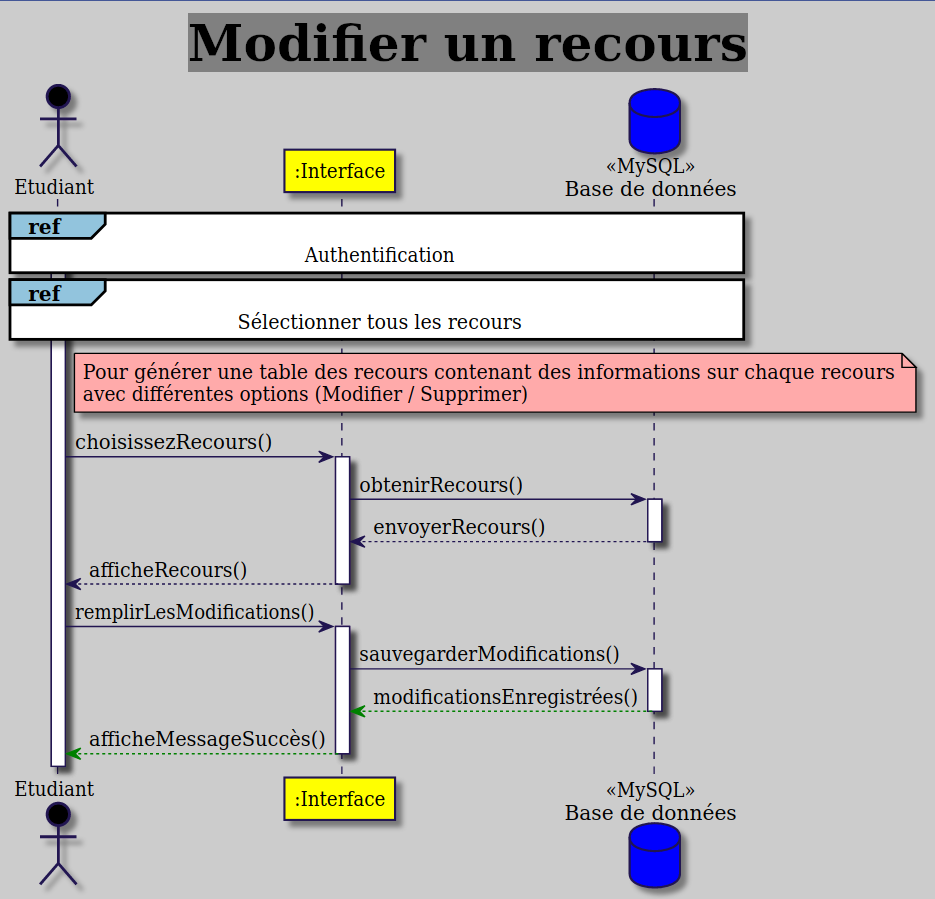
\includegraphics[width = 6.6in, height = 6.2in]{../Conception/Sequence/PNG/Etudiant/ModifierRecours.png}}}
    \caption{Diagramme de séquences <<Modifier un recours>>}
\end{figure}

\vspace{0.2in}

\textbf{Description :}

\begin{itemize}
    \item L'étudiant doit d'abord s'authentifier.
    \item Le système affichera un tableau de ses recours.
    \item L'étudiant choisira un recours à modifier et remplir les modifications.
    \item Le système enregistrera les nouvelles modifications <<requête SQL UPDATE>> et affichera un message de réussite.
\end{itemize}

\newpage

\begin{figure}[h]
\centering
    \centerline{\fbox{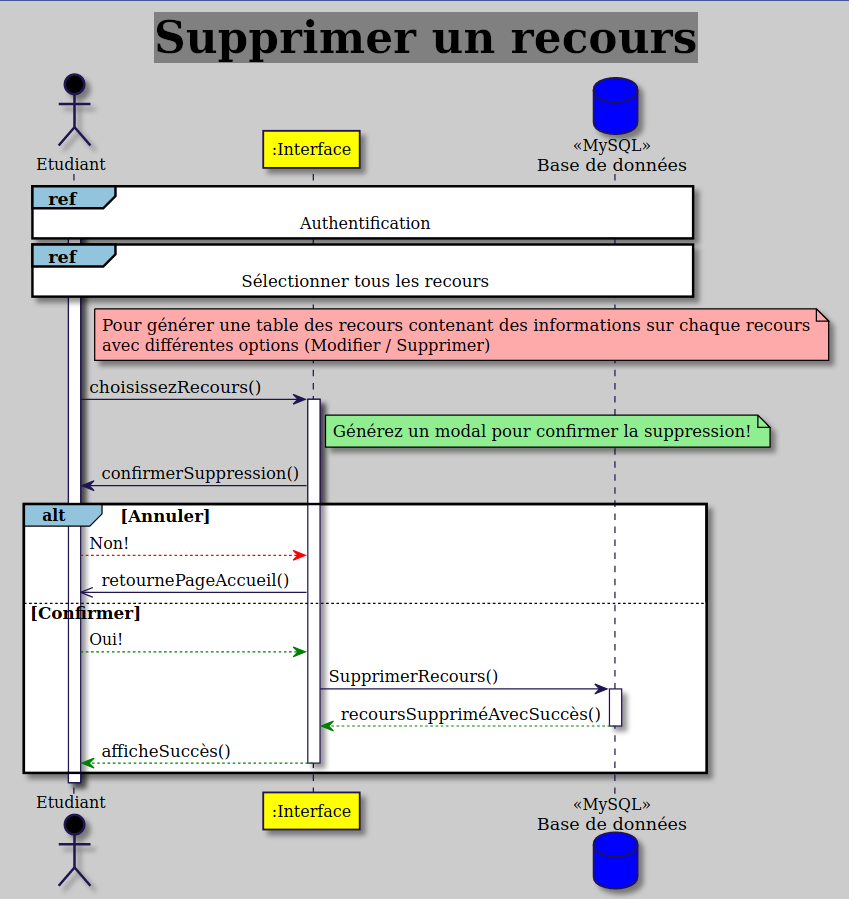
\includegraphics[width = 6.6in, height = 6.2in]{../Conception/Sequence/PNG/Etudiant/SupprimerRecours.png}}}
    \caption{Diagramme de séquences <<Supprimer un recours>>}
\end{figure}

\vspace{0.2in}

\textbf{Description :}

\begin{itemize}
    \item L'étudiant doit d'abord s'authentifier.
    \item Le système affichera un tableau de ses recours.
    \item L'étudiant choisira un recours à modifier et remplir les modifications.
    \item Le système générera un modal CSS pour la confirmation de suppression de recours pour que l'étudiant confirme la suppression.
\end{itemize}

\newpage

\begin{figure}[h]
\centering
    \centerline{\fbox{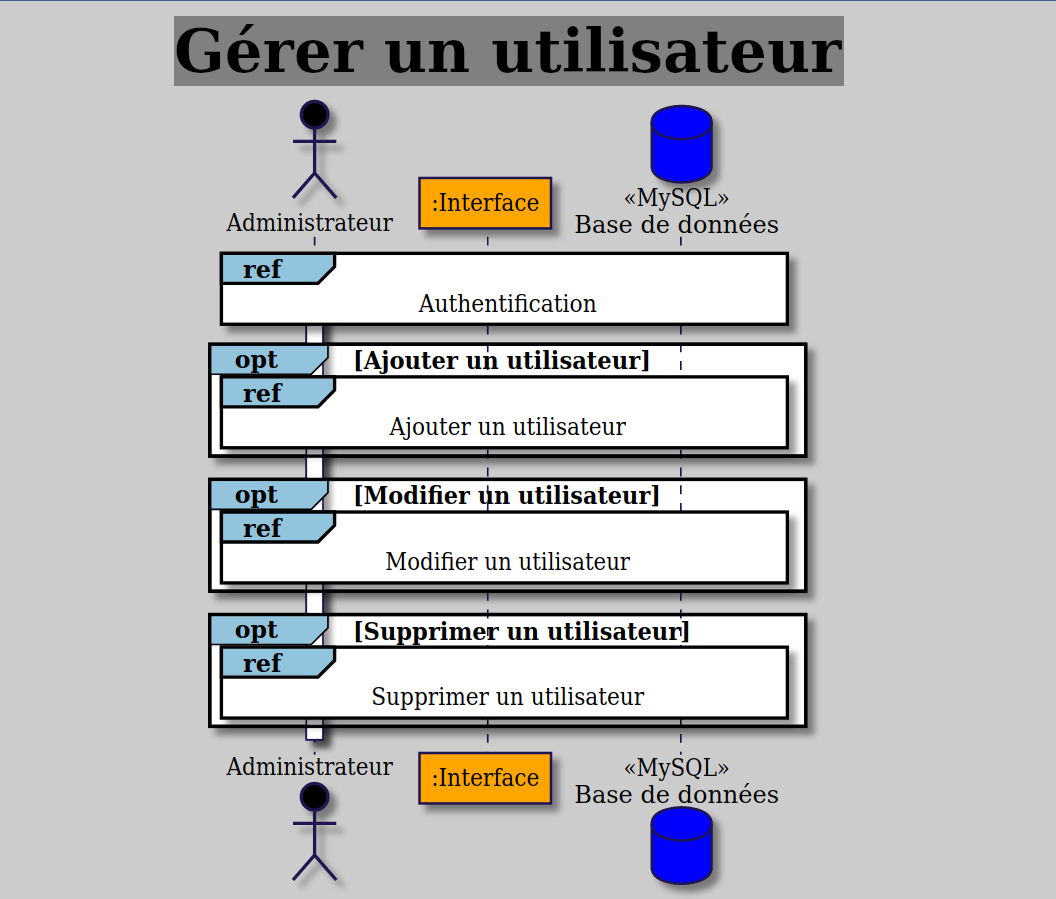
\includegraphics[width = 6.6in, height = 6.2in]{../Conception/Sequence/PNG/Administrateur/Administrateur.png}}}
    \caption{Diagramme de séquences <<G\'erer un utilisateur>>}
\end{figure}

\vspace{0.3in}

\textbf{Description :}

\begin{itemize}
    \item L'administrateur doit d'abord s'authentifier.
    \item L'administrateur peut choisir entre ces options :
    \begin{itemize}
        \item L'ajout d'un utilisateur.
        \item La modification d'un utilisateur.
        \item La suppression d'un utilisateur.
    \end{itemize}
\end{itemize}

\newpage

\begin{figure}[h]
\centering
    \centerline{\fbox{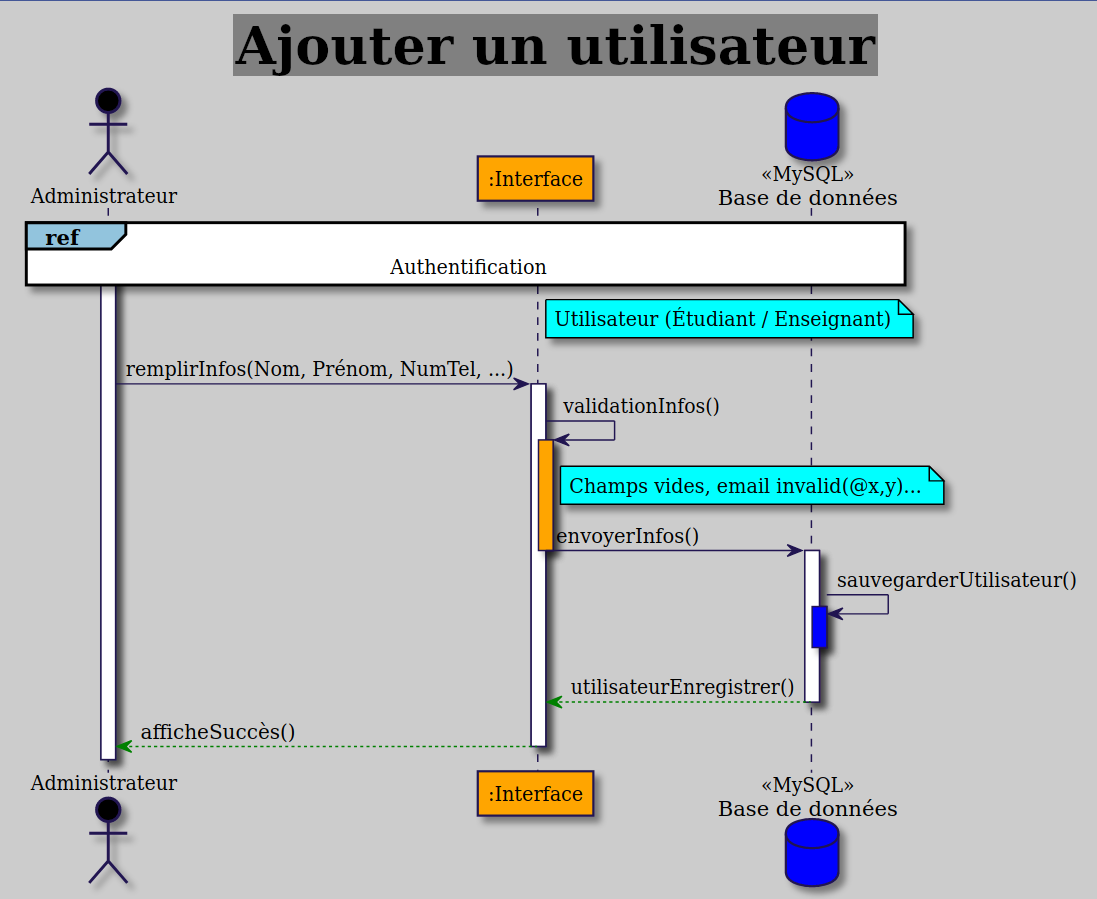
\includegraphics[width = 6.6in, height = 6.2in]{../Conception/Sequence/PNG/Administrateur/AjouterUtilisateur.png}}}
    \caption{Diagramme de séquences <<Ajouter un utilisateur>>}
\end{figure}

\vspace{0.3in}

\textbf{Description :}

\begin{itemize}
    \item L'administrateur doit d'abord s'authentifier.
    \item L'administrateur saisira les informations.
    \item Le système vérifiera les informations fournies.
    \item Enregistrez dans la base de données et affichez le message de réussite.
\end{itemize}

\newpage

\begin{figure}[h]
\centering
    \centerline{\fbox{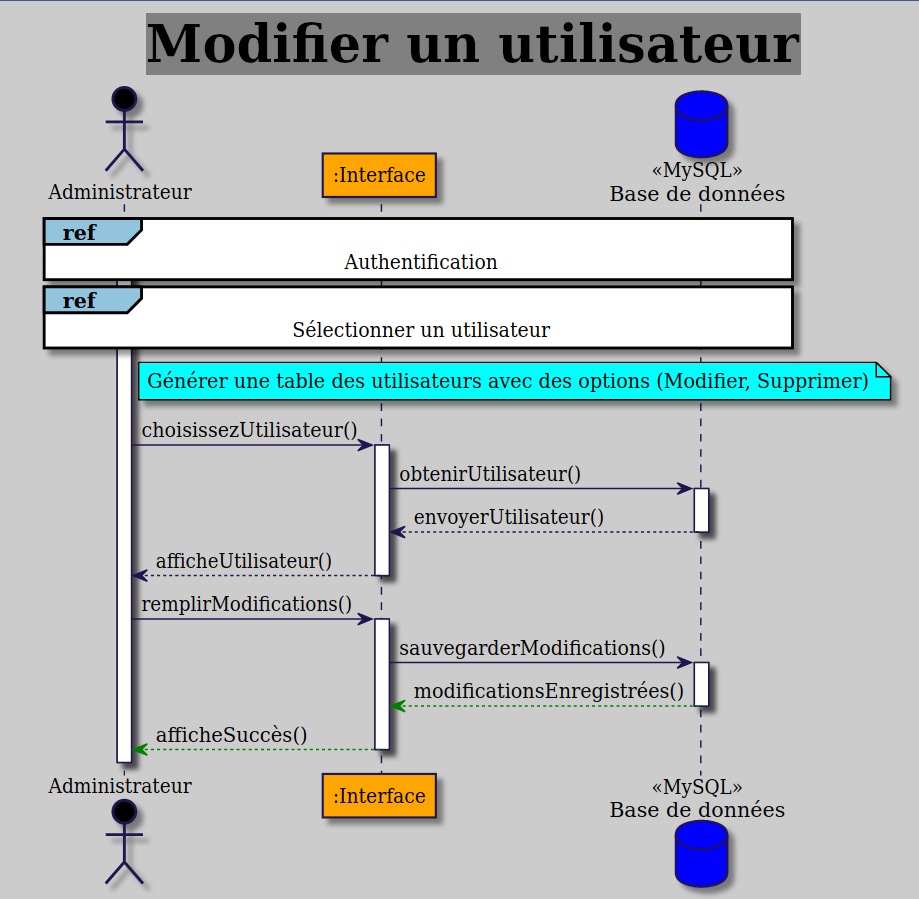
\includegraphics[width = 6.6in, height = 6.2in]{../Conception/Sequence/PNG/Administrateur/ModifierUtilisateur.png}}}
    \caption{Diagramme de séquences <<Modifier un utilisateur>>}
\end{figure}

\vspace{0.3in}

\textbf{Description :}

\begin{itemize}
    \item L'administrateur doit d'abord s'authentifier.
    \item Le système affichera un tableau des utilisateurs.
    \item L'administrateur choisira l'utilisateur et modifiera ses informations.
    \item Le système enregistrera dans la base de données via une requête SQL et affichera un message de réussite.
\end{itemize}

\newpage

\begin{figure}[h]
\centering
    \centerline{\fbox{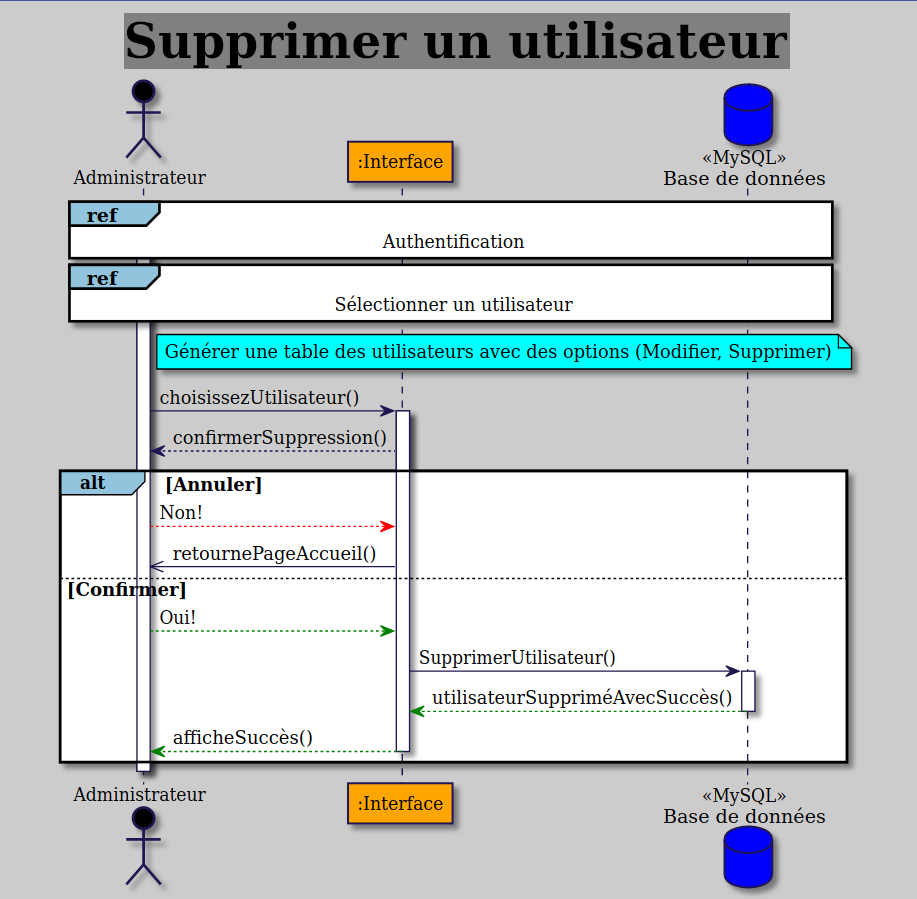
\includegraphics[width = 6.6in, height = 6.2in]{../Conception/Sequence/PNG/Administrateur/SupprimerUtilisateur.png}}}
    \caption{Diagramme de séquences <<Supprimer un utilisateur>>}
\end{figure}

\vspace{0.3in}

\textbf{Description :}

\begin{itemize}
    \item L'administrateur doit d'abord s'authentifier.
    \item Le système affichera un tableau des utilisateurs.
    \item L'administrateur choisira un utilisateur à supprimer.
    \item Le système générera un modal CSS pour confirmer la suppression.
\end{itemize}

\newpage

\subsection{Diagrammes d'activité}

Les diagrammes d'activités sont des représentations graphiques des flux de travail d'activités et d'actions
par étapes avec prise en charge du choix, de l'itération et de la concurrence.
Dans le langage de modélisation unifié, les diagrammes d'activités sont destinés à modéliser
à la fois les processus informatiques et organisationnels (c'est-à-dire les flux de travail),
ainsi que le flux de données qui se croisent avec les activités associées. Bien que les
diagrammes d'activités montrent principalement le flux global de contrôle, ils peuvent
également inclure des éléments montrant le flux de données entre les activités via un ou
plusieurs magasins de données.
\\
Les diagrammes d'activités sont construits à partir d'un nombre limité de formes, relié par des flèches. Les types de formes les plus importants :
\begin{itemize}
    \item les ellipses représentent des actions.
    \item les diamants représentent des décisions.
    \item les barres représentent le début (fractionnement) ou la fin (jointure) des activités simultanées.
    \item un cercle noir représente le début (nœud initial) du flux de travail.
    \item un cercle noir encerclé représente la fin (nœud final).
\end{itemize}
Les flèches vont du début à la fin et représentent l'ordre dans lequel les activités se déroulent.

\begin{figure}[h]
\centering
    \centerline{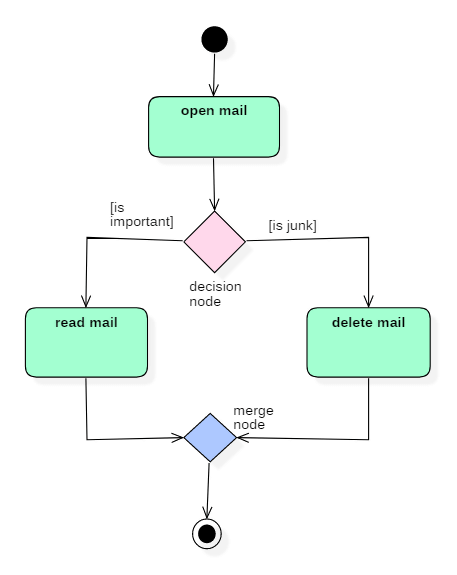
\includegraphics[width = 4.5in, height = 3.7in]{../Images/DiagActEX.png}}
    \caption{Exemple de diagramme d'activité}
\end{figure}

\newpage

\subsubsection{Diagramme d'activité de l'authentification}

\vspace{0.3in}

\begin{figure}[h]
\centering
    \centerline{\fbox{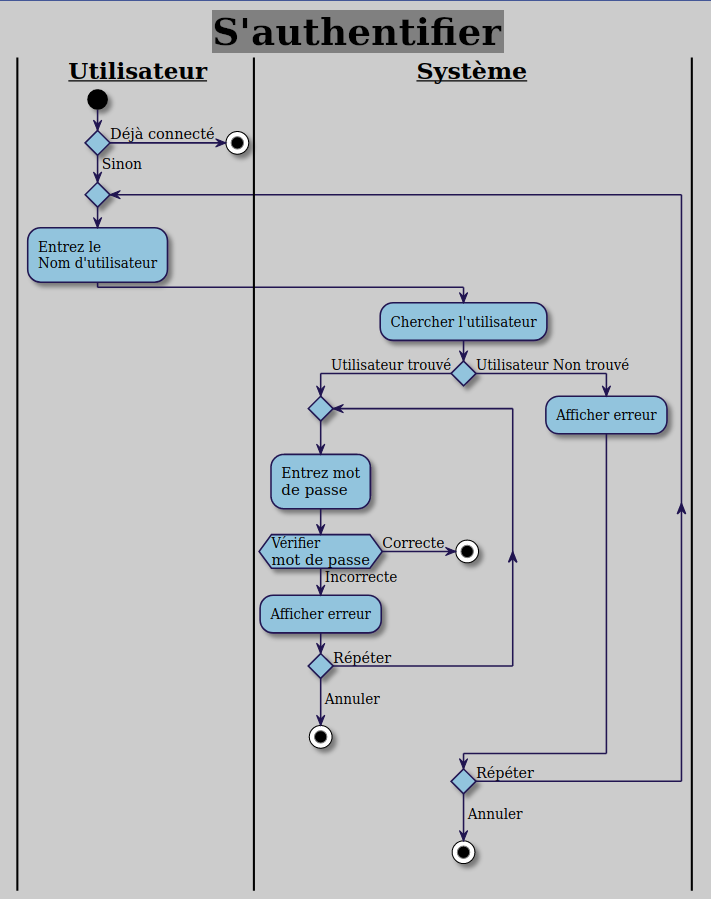
\includegraphics[width = 6.6in, height = 7.2in]{../Conception/Activity/PNG/Authentification.png}}}
    \caption{Diagramme d'activité <<Authentification>>}
\end{figure}

\newpage

\subsubsection{Diagramme d'activité de l'administrateur}

\vspace{0.3in}

\begin{figure}[h]
\centering
    \centerline{\fbox{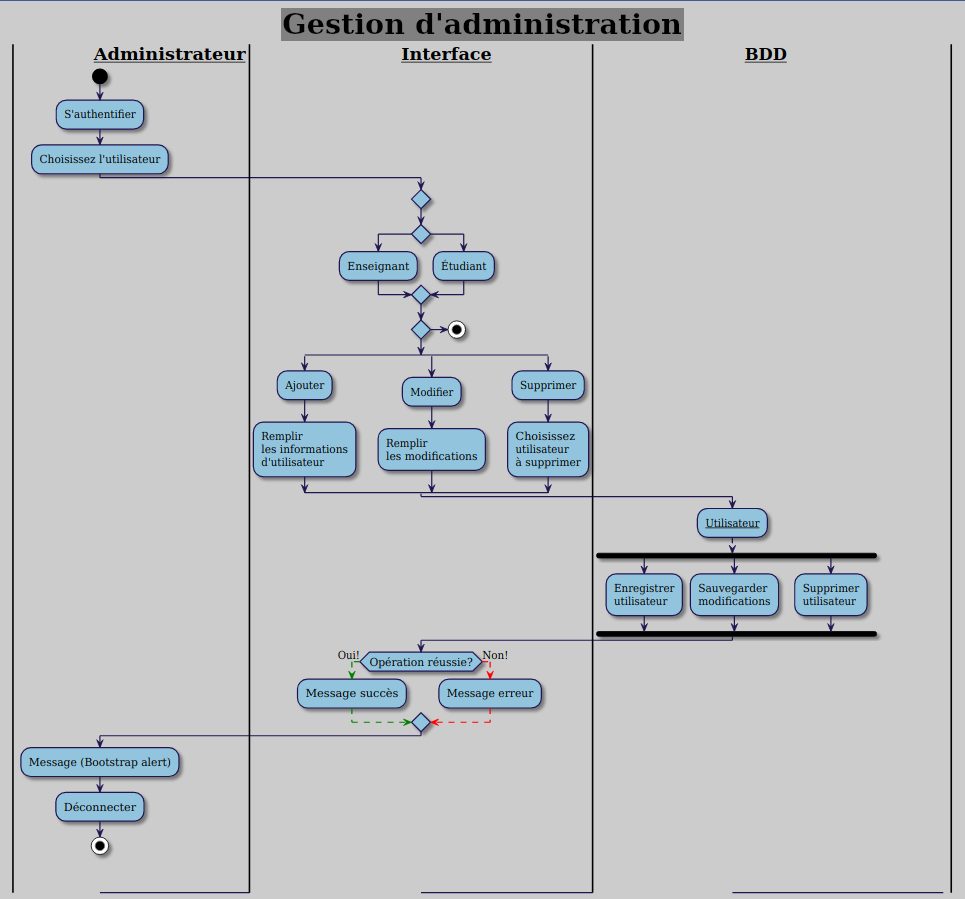
\includegraphics[width = 6.6in, height = 7.2in]{../Conception/Activity/PNG/Administrateur.png}}}
    \caption{Diagramme d'activité <<Administrateur>>}
\end{figure}

\newpage

\subsubsection{Diagramme d'activité de l'enseignant}

\vspace{0.3in}

\begin{figure}[h]
\centering
    \centerline{\fbox{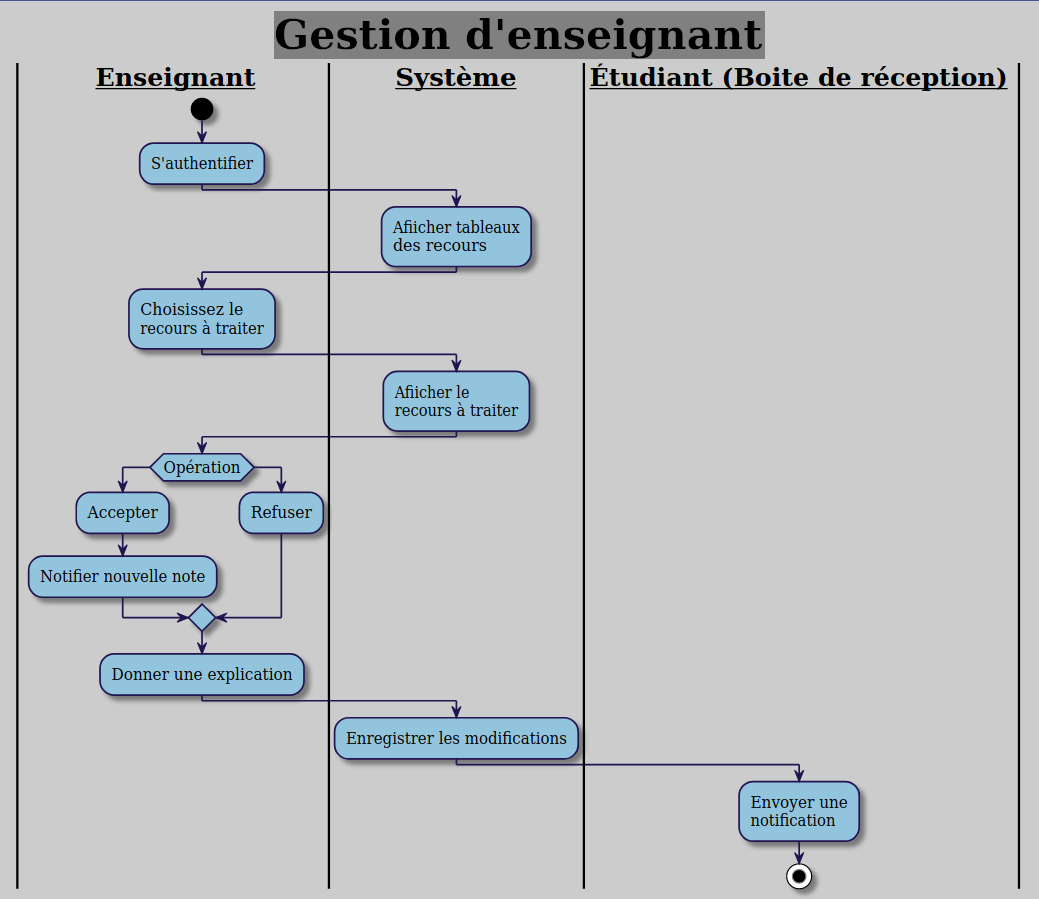
\includegraphics[width = 6.6in, height = 7.2in]{../Conception/Activity/PNG/Enseignant.png}}}
    \caption{Diagramme d'activité <<Enseignant>>}
\end{figure}

\newpage

\subsubsection{Diagramme d'activité de l'étudiant}

\vspace{0.3in}

\begin{figure}[h]
\centering
    \centerline{\fbox{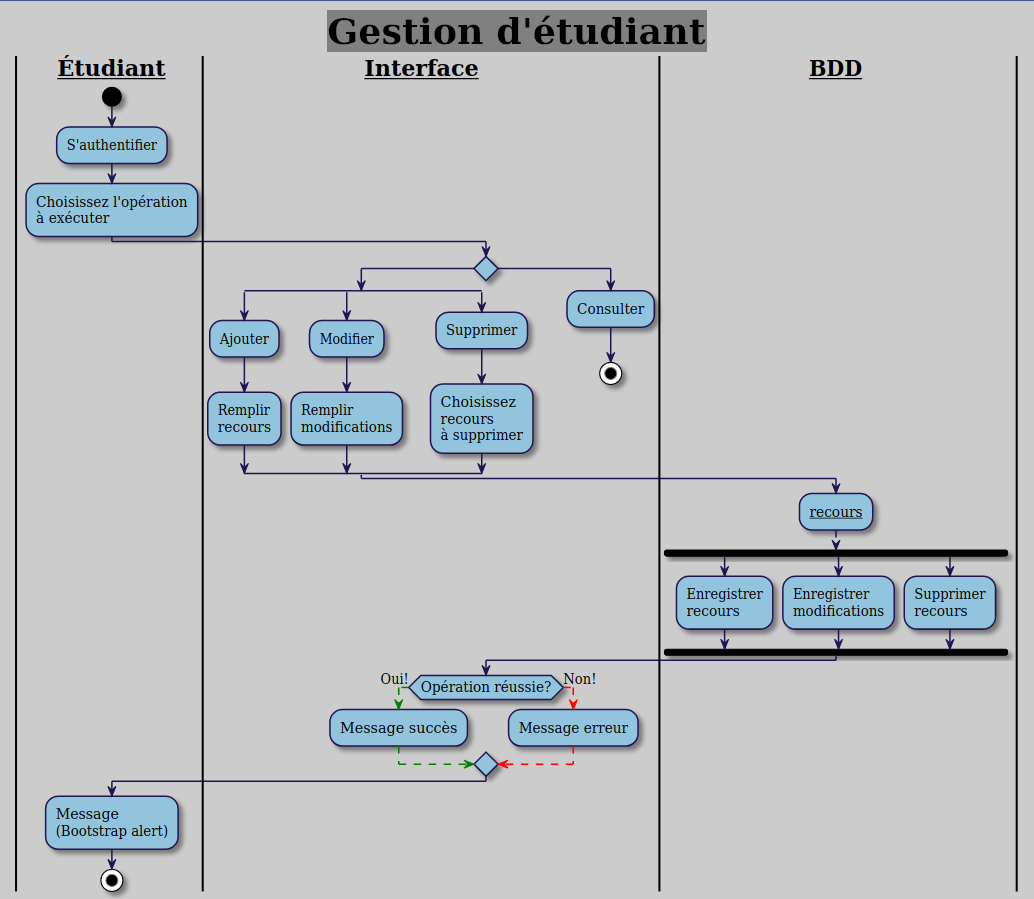
\includegraphics[width = 6.6in, height = 7.2in]{../Conception/Activity/PNG/Etudiant.png}}}
    \caption{Diagramme d'activité <<Étudiant>>}
\end{figure}

\newpage

\subsection{Diagramme de déploiement}

Un diagramme de déploiement dans le langage de modélisation unifié modélise le déploiement physique des artefacts sur les nœuds. Pour décrire un site Web, par exemple, un diagramme de déploiement montrerait quels composants matériels («nœuds») existent (par exemple, un serveur Web, un serveur d’applications et un serveur de base de données), sur quels composants logiciels («artefacts») s’exécutent chaque nœud (par exemple, application Web, base de données), et comment les différentes pièces sont connectées (par exemple JDBC, REST, RMI).
\\
Les nœuds apparaissent sous forme de cases et les artefacts alloués à chaque nœud apparaissent sous forme de rectangles dans les cases. Les nœuds peuvent avoir des sous-nœuds, qui apparaissent comme des boîtes imbriquées. Un seul nœud dans un diagramme de déploiement peut représenter conceptuellement plusieurs nœuds physiques, tels qu'un cluster de serveurs de base de données.

\vspace{0.2in}

\subsubsection{Le diagramme de déploiement}

\vspace{0.2in}

\begin{figure}[h]
\centering
    \centerline{\fbox{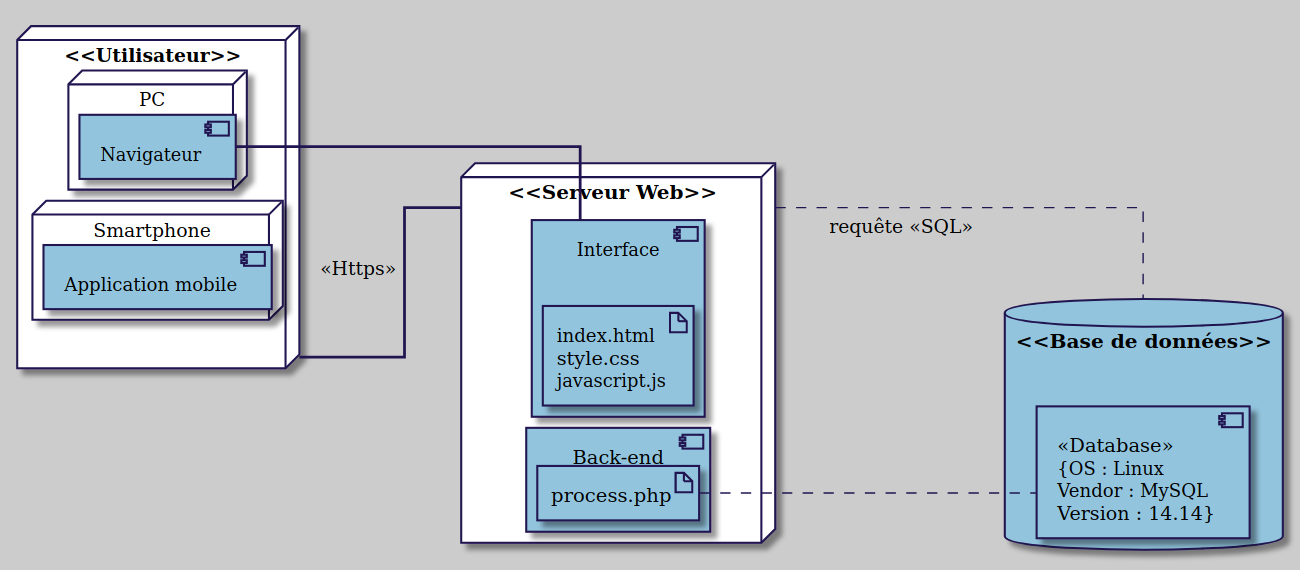
\includegraphics[width = 6.6in, height = 4in]{../Conception/Deployment/PNG/Deployment.png}}}
    \caption{Diagramme de déploiement}
\end{figure}

\newpage

\subsection{Diagrammes des classes}

En génie logiciel, un diagramme de classes dans le langage de modélisation unifié (UML) est un type de diagramme de structure statique qui décrit la structure d'un système en montrant les classes du système, leurs attributs, opérations (ou méthodes) et les relations entre les objets.
\\\\
Le diagramme de classes est le principal bloc de construction de la modélisation orientée objet. Il est utilisé pour la modélisation conceptuelle générale de la structure de l'application et pour la modélisation détaillée traduisant les modèles en code de programmation. Les diagrammes de classes peuvent également être utilisés pour la modélisation des données. Les classes d'un diagramme de classes représentent à la fois les éléments principaux, les interactions dans l'application et les classes à programmer.

\vspace{0.1in}

\subsubsection{Diagramme de classe Général}

\vspace{0.1in}

\begin{figure}[h]
\centering
    \centerline{\fbox{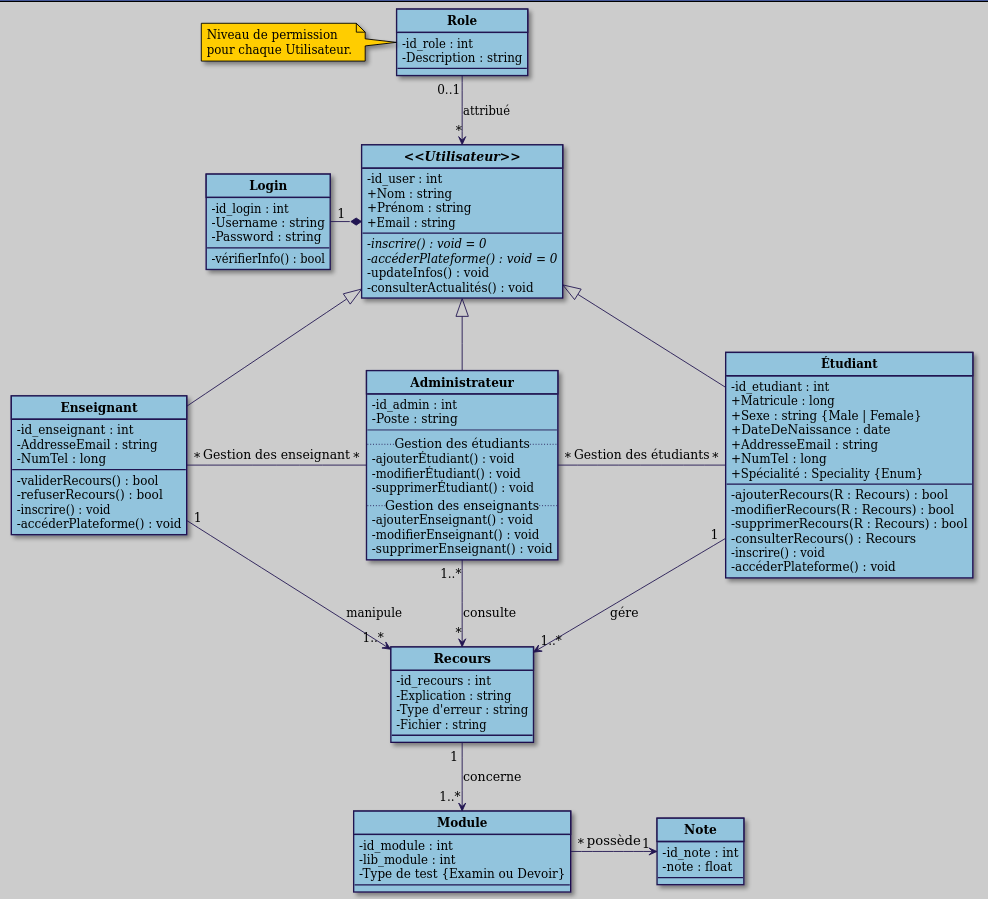
\includegraphics[width = 6.6in, height = 5in]{../Conception/Class/PNG/Utilisateur.png}}}
    \caption{Diagramme de classe <<Utilisateur>>}
\end{figure}

\textbf{\uline{Remarque}} : Les diagrammes détaillés sont ci-dessous pour tous les acteurs.

\newpage

\subsubsection{Diagramme de classe pour l'administrateur}

\begin{figure}[h]
\centering
    \centerline{\fbox{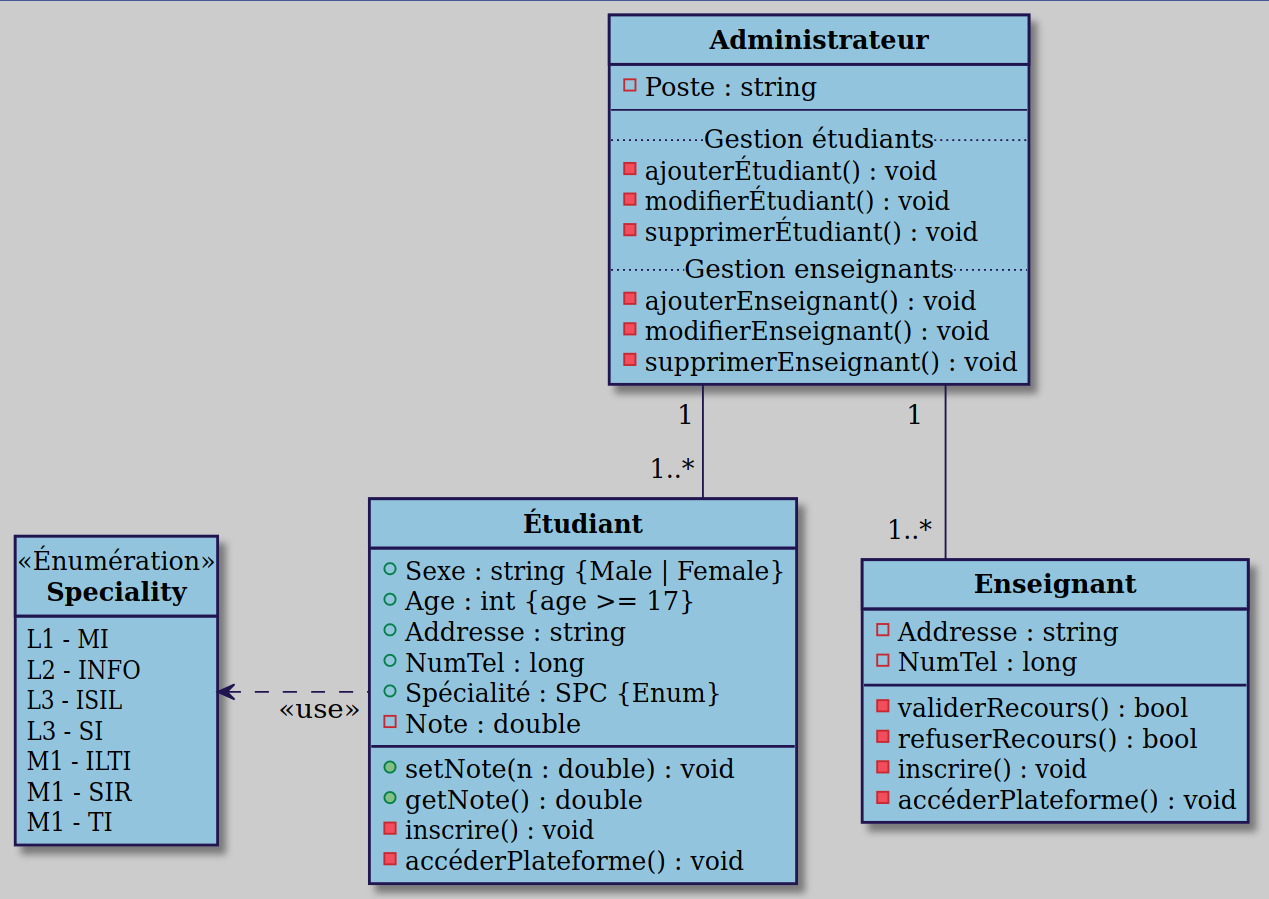
\includegraphics[width = 6.6in, height = 5in]{../Conception/Class/PNG/Administrateur.png}}}
    \caption{Diagramme de classe <<Administrateur>>}
\end{figure}

\vspace{0.3in}

\textbf{Description :}

\begin{itemize}
    \item L'administrateur a le choix entre plusieurs options pour gérer les utilisateurs (étudiants et enseignants) :
    \begin{itemize}
        \item Ajouter.
        \item Modifier.
        \item Supprimer.
    \end{itemize}
    \item Il peut gérer un ou plusieurs utilisateurs.
    \item Les utilisateurs (étudiants et enseignants) peuvent être gérés par un seul administrateur.
\end{itemize}

\newpage

\subsubsection{Diagramme de classe pour l'enseignant}

\begin{figure}[h]
\centering
    \centerline{\fbox{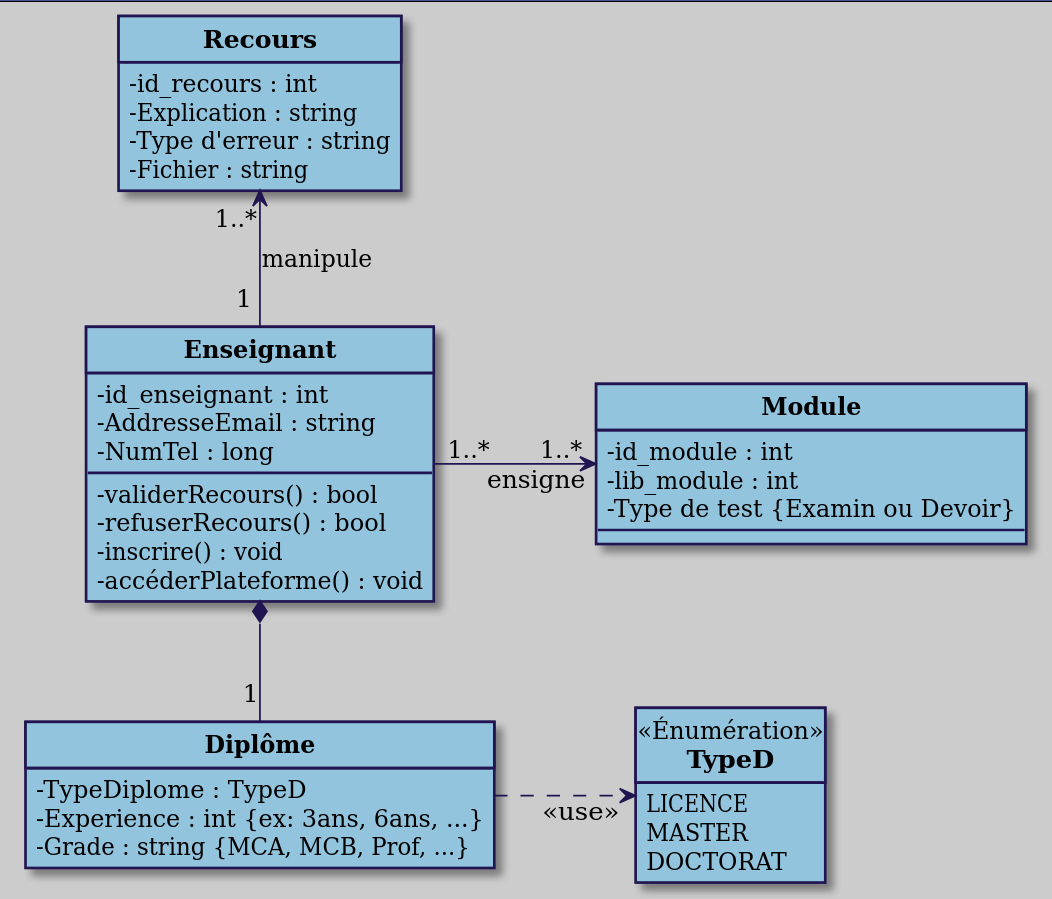
\includegraphics[width = 6.6in, height = 6.2in]{../Conception/Class/PNG/Enseignant.png}}}
    \caption{Diagramme de classe <<Enseignant>>}
\end{figure}

\vspace{0.3in}

\textbf{Description :}

\begin{itemize}
    \item L'enseignant a un 'Grade' comme option supplémentaire pour déterminer le niveau de privilège dont il dispose.
    \item L'enseignant peut valider ou refuser un ou plusieurs recours soumis par les étudiants et il peut également s'inscrire.
    \item L'enseignant est composé d'un diplôme et la classe diplôme utilise l'énumération TypeD pour déterminer son type.
\end{itemize}

\newpage

\subsubsection{Diagramme de classe pour l'étudiant}

\begin{figure}[h]
\centering
    \centerline{\fbox{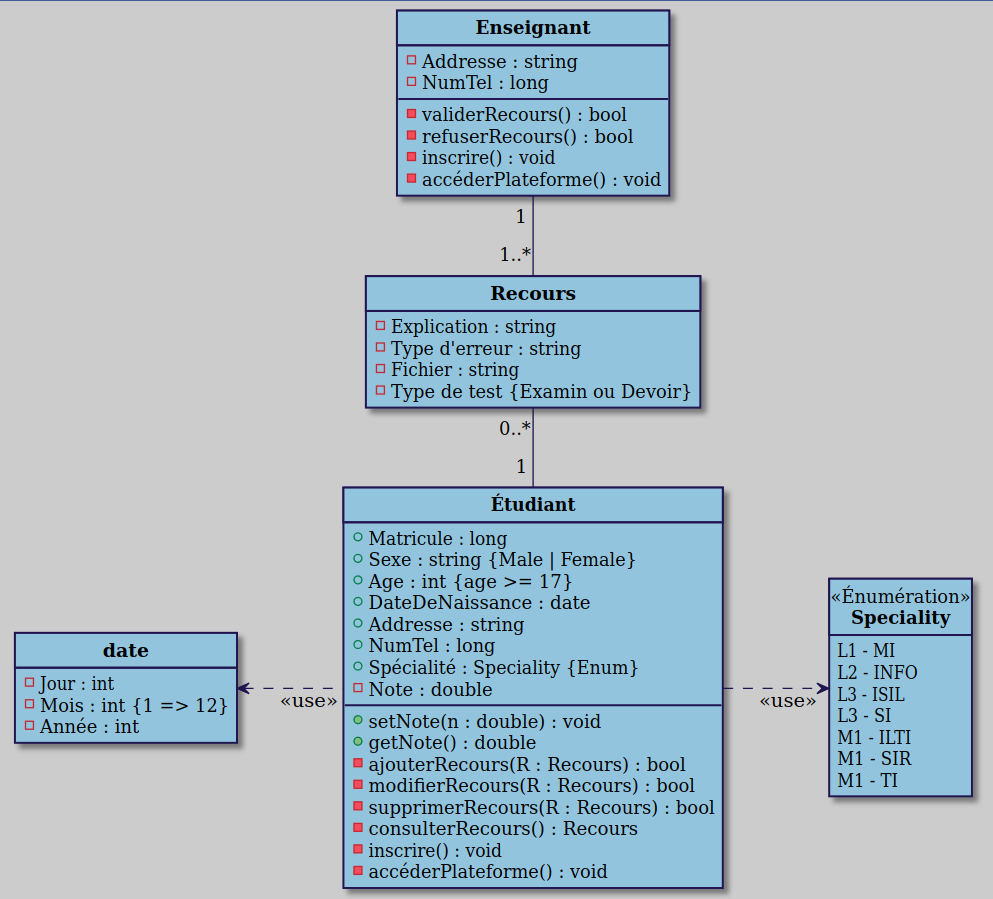
\includegraphics[width = 6.6in, height = 6.2in]{../Conception/Class/PNG/Etudiant.png}}}
    \caption{Diagramme de classe <<Étudiant>>}
\end{figure}

\vspace{-0.1in}

\textbf{Description :}

\vspace{-0.1in}
\begin{itemize}
    \item L'étudiant peut manipuler ses recours et peut également joindre un fichier (Code, explication...)
\end{itemize}

\vspace{-0.4in}

\section{Conclusion}
Dans ce chapitre, nous avons défini d'abord la signification de l'analyse et la conception avec les outils que on a utilisés pour réussir notre conception, Ensuite nous sommes passés au différents diagrammes (Cas d'utilisation, Activité, Séquence...) la où nous avons expliqué notre solution en détail. Cette étude nous a permis de définir la structure de l’application et cela aussi nous a facilité l’implémentation que vous verraient dans le chapitre suivant.

\newpage

\vspace*{\fill}
\begin{center}
    {\color{Blue} \rule{\linewidth}{1.2mm} }\\
\vspace{0.25in}
    {\centering\fontsize{30}{40}{\bfseries{\color{Blue}{\scshape{Chapitre III : Réalisation}}}}}
\vspace{0.35in}\\
    {\color{Blue} \rule{\linewidth}{1.2mm} }
\end{center}
\vspace*{\fill}
\addcontentsline{toc}{chapter}{\color{Blue}{Chapitre III : Réalisation}}
\setcounter{section}{0}

\newpage

\section{Introduction}

Enfin, la phase de la réalisation, c'est là que nous allons devenir très technique, nous allons utiliser diverses des technologies (Chartjs, JQuery, Ajax, PDO...) et divers outils comme (Vim, mycli...) pour nous aider dans notre workflow, la sécurité est également une partie cruciale du développement et nous allons donc vérifier chaque champ d'entrée avec ses conditions (spéciales) appropriées et garder un œil sur la partie des téléchargements de fichiers (Images,...), le tout avec tant de petites choses pour améliorer la sécurité.
\\\\
Nous allons creuser profondément dans le backend et le frontend et comment nous avons tout fait fonctionner à partir de zéro.

\section{Les langages de programmation utilisés}

\subsection{HTML}

Hyper Text Markup Language (HTML) est le langage de balisage standard pour les documents conçus pour être affichés dans un navigateur Web. Il peut être assisté par des technologies telles que les feuilles de style en cascade (CSS) et des langages de script tels que JavaScript.
Les navigateurs Web reçoivent des documents HTML d'un serveur Web ou d'un stockage local et convertissent les documents en pages Web multimédias. HTML décrit la structure d'une page Web de manière sémantique et inclut à l'origine des indices pour l'apparence du document.

\vspace{0.6in}

\begin{figure}[h]
\centering
    
\includegraphics[width = 3.2in, height = 2.4in]{../Images/Html.png}
\caption{Logo HTML}
\end{figure}

\newpage

\subsection{CSS}

Cascading Style Sheets (CSS) est un langage de feuille de style utilisé pour décrire la présentation d'un document écrit dans un langage de balisage comme HTML. CSS est une technologie de base du World Wide Web, avec HTML et JavaScript.
\\
CSS est conçu pour permettre la séparation de la présentation et du contenu, y compris la mise en page, les couleurs et les polices. Cette séparation peut améliorer l'accessibilité du contenu, fournir plus de flexibilité et de contrôle dans la spécification des caractéristiques de présentation, permettre à plusieurs pages Web de partager le formatage en spécifiant le CSS pertinent dans un fichier .css séparé, ce qui réduit la complexité et la répétition dans le contenu structurel et permet le fichier .css à mettre en cache pour améliorer la vitesse de chargement des pages entre les pages qui partagent le fichier et son formatage.

\vspace{0.22in}

\begin{figure}[h]
\centering
    
\includegraphics[width = 2.3in, height = 2.6in]{../Images/CSS.png}
\caption{Logo CSS}
\end{figure}

\subsection{Bootstrap}

Bootstrap est un framework CSS gratuit et open-source destiné au développement Web frontal réactif et mobile. Il contient des modèles de conception basés sur CSS et (éventuellement) JavaScript pour la typographie, les formulaires, les boutons, la navigation et d'autres composants d'interface.

\begin{figure}[h]
\centering
    \includegraphics[width = 3.5in, height = 1.3in]{../Images/Bootstrap.png}
\vspace{-0.2in}
\caption{Logo Bootstrap}
\end{figure}

\newpage

\subsection{Javascript}

JavaScript, souvent abrégé en JS, est un langage de programmation conforme à la spécification ECMAScript. JavaScript est de haut niveau, souvent compilé juste à temps et multi-paradigme. Il a une syntaxe entre crochets, un typage dynamique, une orientation d'objet basée sur un prototype et des fonctions de première classe.
\\
JavaScript est l'une des technologies de base du World Wide Web.
\\
Nous avons utilisé javascript principalement pour la validation des utilisateurs côté client et certaines animations pour un site Web plus beau.

%\vspace{-0.2in}

\begin{figure}[h]
\centering
    \includegraphics[width = 2.8in, height = 2.6in]{../Images/JS.png}
\caption{Logo Javascript}
\end{figure}

\vspace{-0.18in}

\subsection{PHP}

PHP est un langage de script à usage général qui est particulièrement adapté au développement Web. Il a été créé à l'origine par le programmeur danois-canadien Rasmus Lerdorf en 1994, l'implémentation de référence PHP est maintenant produite par The PHP Group. PHP signifiait à l'origine Personal Home Page, mais il représente maintenant l'initialisme récursif PHP : Hypertext Preprocessor.
\\
Il a été utilisé pour manipuler le code HTML CSS et MySQL pour établir des relations entre la base de données et la page Web principale.

\vspace{-0.2in}

\begin{figure}[h]
\centering
    \includegraphics[width = 2.8in, height = 2.0in]{../Images/PHP.png}
\vspace{-0.3in}
\caption{Logo PHP}
\end{figure}

\newpage

\subsection{MySQL}

MySQL est un système de gestion de base de données relationnelle (SGBDR) open source. Son nom est une combinaison de "My", le nom de la fille du co-fondateur Michael Widenius, et "SQL", l'abréviation de Structured Query Language. Une base de données relationnelle organise les données en une ou plusieurs tables de données dans lesquelles les types de données peuvent être liés les uns aux autres, ces relations aident à structurer les données.
\\
SQL est un langage utilisé par les programmeurs pour créer, modifier et extraire des données de la base de données relationnelle, ainsi que pour contrôler l'accès des utilisateurs à la base de données. En plus des bases de données relationnelles et SQL, un SGBDR comme MySQL fonctionne avec un système d'exploitation pour implémenter une base de données relationnelle dans le système de stockage d'un ordinateur, gère les utilisateurs, permet l'accès au réseau et facilite les tests de l'intégrité de la base de données et la création de sauvegardes.
\\\\
MySQL est un logiciel libre et open source sous les termes de la licence publique générale GNU, et est également disponible sous une variété de licences propriétaires. MySQL était détenu et sponsorisé par la société \\suédoise MySQL AB, qui a été rachetée par Sun Microsystems (aujourd'hui Oracle Corporation). En 2010, lors de l'acquisition de Sun par Oracle, Widenius a lancé le projet open source MySQL pour créer MariaDB.

\vspace{0.7in}

\begin{figure}[h]
\centering
    \includegraphics[width = 3.8in, height = 2in]{../Images/MySQL.png}
\vspace{0.1in}
\caption{Logo MySQL}
\end{figure}

\newpage

\section{Les outils utilisés}

\subsection{Vim}

Vim, l'éditeur de texte de choix, c'est un éditeur de texte très rapide et fiable qui aide beaucoup en termes de flux de travail et pour couronner le tout, il a divers plugins qui aident tellement avec tout travail qui doit être fait, pour cela section du développement Web, nous avons utilisé des plugins comme Syntastic pour générer des erreurs de syntaxe en temps réel et YouCompletMe pour une auto-complétion de code facile, également Emmet pour générer des extraits (Code Snippets) comme des balises HTML en très peu de clics de clavier, et bien d'autres plugins...

\vspace{0.1in}

\begin{figure}[h]
\centering
    \includegraphics[width = 3in, height = 2in]{../Images/Vim.png}
\vspace{0.0in}
\caption{Logo Vim}
\end{figure}

\vspace{-0.15in}

\subsection{Mycli}

MyCLI est une interface de ligne de commande pour MySQL, MariaDB et Percona avec complétion automatique et coloration syntaxique. Il est utilisé pour coder le code MySQL car il dispose de la mise en évidence des couleurs et de l'auto-complétion afin que nous puissions voir et essayer différentes commandes dans la ligne de commande, comme indiqué dans l'image ci-dessous :

\begin{figure}[h]
\centering
    \includegraphics[width = 6in, height = 2.4in]{../Images/mycli.png}
\vspace{-0.1in}
\caption{Exemple Mycli}
\end{figure}

\newpage

\subsection{Apache}

Le serveur HTTP Apache, familièrement appelé Apache, est un logiciel de serveur Web multiplateforme gratuit et open source, publié sous les termes de la licence Apache 2.0. Apache est développé et maintenu par une communauté ouverte de développeurs sous les auspices de l'Apache Software Foundation.
\\
La grande majorité des instances Apache HTTP Server fonctionnent sur une distribution Linux, mais les versions actuelles fonctionnent également sur Microsoft Windows et une grande variété de systèmes de type Unix. Les versions précédentes fonctionnaient également sur OpenVMS, NetWare, OS / 2 et d'autres systèmes d'exploitation, y compris les ports vers les mainframes.
\\
Utilisé pour afficher notre page Web dans un navigateur (Chrome principalement) pour configurer l'hébergement local (Localhost)

\begin{figure}[h]
\centering
    \includegraphics[width = 3.4in, height = 1.3in]{../Images/Apache.png}
\caption{Logo Apache}
\end{figure}

\subsection{PhpMyAdmin}

PhpMyAdmin est un outil d'administration gratuit et open source pour MySQL et MariaDB, En tant qu'application Web portable écrite principalement en PHP, elle est devenue l'un des outils d'administration MySQL les plus populaires, en particulier pour les services d'hébergement Web (Web hosting).

\vspace{0.2in}

\begin{figure}[h]
\centering
    \includegraphics[width = 3.4in, height = 2in]{../Images/PhpMyAdmin.png}
\caption{Logo PhpMyAdmin}
\end{figure}

\newpage

\section{Architecture}

Pour nous aider à construire un site Web bien formé, nous avons choisi d'adopter MVC :
\\\\
Model - View - Controller (généralement connu sous le nom de MVC) est un modèle de conception de logiciel couramment utilisé pour développer des interfaces utilisateur qui divise la logique de programme associée en trois éléments inter-connectés. Ceci est fait pour séparer les représentations internes des informations de la manière dont les informations sont présentées et acceptées par l'utilisateur. Ce type de motif est utilisé pour concevoir la mise en page de la page.
\\\\
Traditionnellement utilisé pour les interfaces utilisateur graphiques (GUIs) de bureau, ce modèle est devenu populaire pour la conception d'applications Web. Les langages de programmation populaires tels que JavaScript, Python, Ruby, PHP, Java, C\# et Swift ont des frameworks MVC qui sont utilisés pour le développement d'applications Web ou mobiles dès la sortie de la boîte.

\vspace{0.5in}

\begin{figure}[h]
\centering
    \includegraphics[width = 4.0in, height = 4.2in]{../Images/MVC.png}
\caption{Architecture MVC}
\end{figure}

\newpage

\section{Matériaux utilisés}

Voici les matériaux que nous avons utilisés pour créer le site Web avec github pour nous aider en termes de synchronisation (à jour) :

\subsection{Environnement matériel}

\vspace{0.1in}

\begin{table}[h]
  \centering
  \large
\begin{tabular}{|c|l|}
\hline
\rowcolor[HTML]{ECF4FF}
{\color[HTML]{000000} \textbf{Le matériel}} & \multicolumn{1}{c|}{\cellcolor[HTML]{ECF4FF}{\color[HTML]{000000} \textbf{Caractéristiques}}}                                                                                                                                                                                                            \\ \hline
\rowcolor[HTML]{DAE8FC}
{\color[HTML]{000000} \textbf{PC 1}}        & {\color[HTML]{000000} \begin{tabular}[c]{@{}l@{}}Brand : Apple\\ Model : MacBook Air (13-inch, Mid 2013)\\ RAM : 4GB 1600MHz LPDDR3\\ CPU : Intel Core i5 1.3GHz dual-core (2.6GHz TB)\\ GPU : Intel HD Graphics 5000\\ OS : Linux Mint 19.2 Tina\\ Storage : 128GB flash storage (SSD)\end{tabular}} \\ \hline
\rowcolor[HTML]{ECF4FF}
{\color[HTML]{000000} \textbf{PC 2}}        & {\color[HTML]{000000} \begin{tabular}[c]{@{}l@{}}Brand : Sony\\ Model : Vaio (2015)\\ RAM : 4 GB 1600MHz LPDDR3\\ CPU : Intel Core i5-2430M 2.4Ghz dual-core\\ GPU : Intel HD Graphics 3000\\ OS : Ubuntu 18.04.4 LTS Bionic Beaver\\ Storage : 128GB flash storage (HDD)\end{tabular}}                  \\ \hline
\end{tabular}
  \caption{Matériaux}
\end{table}

\subsection{Signification des abréviations}

\vspace{0.2in}

RAM \hspace{0.245in} ==> \hspace{0.22in} Random Access Memory
\\
CPU \hspace{0.3in} ==> \hspace{0.22in} Central Processing Unit
\\
GPU \hspace{0.3in} ==> \hspace{0.22in} Graphical Processing Unit
\\
OS  \hspace{0.42in} ==> \hspace{0.22in} Operating System
\\
SSD \hspace{0.33in} ==> \hspace{0.22in} Solid State Drive
\\
HDD \hspace{0.28in} ==> \hspace{0.22in} Hard Disk Drive
\\
TB  \hspace{0.43in} ==> \hspace{0.22in} Turbo Boost 
\\
LTS \hspace{0.365in} ==> \hspace{0.22in} Long Term Support

\newpage

\section{Le site Web}

\subsection{Page de connexion}

\vspace{0.2in}

Ceci est la première page avec laquelle tout type d'utilisateur va être accueilli, et donc ici nous pouvons identifier les utilisateurs soit par leur `Nom d'utilisateur' ou leur `Email' et `Mot de passe' évidemment pour des raisons de sécurité, sinon si l'utilisateur ne s'est pas encore enregistré, il peut cliquer sur créer un compte et s'inscrire.
\\\\
Les champs d'entrée sont sécurisés à l'aide d'instructions SQL préparées et le mot de passe est haché puis comparé à son équivalent dans la base de données pour vérifier et authentifier l'utilisateur concerné.

\vspace{0.8in}

\begin{figure}[h]
\centering
    \fbox{\includegraphics[width = 6.6in, height = 4.5in]{../Site/login.png}}
\caption{Page de connexion}
\end{figure}

\newpage

\subsection{Page d'inscription}

\vspace{0.2in}

La page d'inscription est la page où tout utilisateur donné peut soit entrer ses coordonnées et enregistrer un nouveau compte, soit revenir à la page de connexion si l'utilisateur a déjà un compte, le formulaire a une sorte de deux facteurs d'authentification puisque nous avons utilisé validation côté client (JavaScript) pour vérifier les longueurs de valeur et si les mots de passe correspondent ou non etc..., également une autre couche de sécurité côté serveur (PHP) pour vérifier si un utilisateur existe déjà et si un mot de passe donné est suffisamment sécurisé, et d'autres petits détails...
\\\\
Les mots de passe sont hachés à l'aide de la dernière version de Bcrypt (algorithme) et toutes les instructions SQL sont préparées afin qu'il n'y ait rien à craindre en termes d'attaques par injection SQL.

\vspace{0.8in}

\begin{figure}[h]
\centering
    \fbox{\includegraphics[width = 6.6in, height = 4.5in]{../Site/register.png}}
\caption{Page d'inscription}
\end{figure}

\newpage

\subsection{Page d'inscription complète}

La dernière page enregistre un nouvel utilisateur toujours en tant que visiteur, et ainsi, dans cette page, un utilisateur peut compléter complètement son enregistrement pour bénéficier de l'utilisation de ce site Web en conséquence, tout comme la dernière page, tous les champs de saisie sont vérifiés en utilisant les deux méthodes mentionnées ci-dessus (validation côté client et côté serveur), et des vérification spécifique par exemple un nom ne peut pas contenir des caractères spéciaux et ainsi de suite..., ici un utilisateur peut spécifier quel type d'utilisateur il / elle, le type d'utilisateur sélectionner générera des champs de saisie spécifiques qui se réfèrent uniquement au type d'utilisateur choisi (en utilisant Ajax) <<Figure 60>>, pour référence :

\begin{itemize}
  \item \textbf{Étudiant} (groupe, spécialité, matricule).
  \item \textbf{Enseignant} (grade, diplôme, matricule).
  \item \textbf{Administrateur} (poste, id).
\end{itemize}

\vspace{0.08in}

\begin{figure}[h]
\centering
    \fbox{\includegraphics[width = 6.6in, height = 4.5in]{../Site/registerFULL.png}}
  \caption{Page d'inscription complète}
\end{figure}

\newpage

\begin{figure}[h]
\centering
    \fbox{\includegraphics[width = 6.6in, height = 4.5in]{../Site/registerFULL2.png}}
  \caption{Page d'inscription complète (Type d'utilisateur)}
\end{figure}

\subsection{Page d'accueil}

Une fois l'enregistrement terminé et réussi, l'utilisateur sera redirigé vers la page d'accueil. Dans cette page, nous avons essayé de le rendre aussi simple que possible et de ne pas effrayer un nouvel utilisateur une fois qu'il s'est enregistré avec succès, il a un style de carte pour rediriger un utilisateur vers diverses autres pages en fonction du type d'utilisateur, par exemple :

\begin{itemize}
  \item \textbf{Visiteur} : une carte pour rediriger vers la page d'inscription complète et une autre pour voir les dernières informations sur les pages du tableau de bord et des graphiques avec un accès minimal.
  \item \textbf{Étudiant} : recommander de manipuler ses recours (Ajouter, Mettre à jour, Supprimer...). sinon, redirigez pour voir les dernières informations du tableau de bord.
  \item \textbf{Enseignant} : recommandation de manipuler les recours soumis par ses élèves.
  \item \textbf{Administrateur} : une carte recommandant de manipuler les utilisateurs (Ajouter, Mettre à jour, Supprimer...)
et une autre pour voir le flux de trafic des recours.
\end{itemize}

\newpage

\begin{figure}[h]
\centering
    \fbox{\includegraphics[width = 6.6in, height = 4.5in]{../Site/index.png}}
\caption{Page d'accueil}
\end{figure}

\subsection{Page de profil pour un étudiant}

Les quatre figures suivantes porteront sur la manière dont un étudiant interagit avec le site, dès qu'un étudiant entre dans cette page, il lui sera présenté une liste de ses recours et certains de leurs détails (module, enseignant concerné, statut...) comme le montre la première figure <<Figure 62>>, un étudiant peut également supprimer ou effectuer une action comme indiqué ci-dessous :

\begin{itemize}
  \item \textbf{Ajouter / Modifier :} un élève peut (ajouter, modifier) un recours en remplissant quelques entrées, il peut également uploader un fichier (code c, c++, asm, js, photo, pdf...) qui est lié au recours pour un recours plus fort, l'enseignant concerné doit être un enseignant valide déjà inscrit. <<Figure 63-64>>
  \item \textbf{Consulter :} ici un étudiant peut consulter tous les détails concernant le recours choisi avec des liens rapides pour le modifier ou le supprimer. <<Figure 65>>
\end{itemize}
\textbf{\uline{Remarque :}} un étudiant ne peut modifier que les recours ayant le statut "En Cours".

\newpage

\begin{figure}[H]
\centering
    \fbox{\includegraphics[width = 6.6in, height = 4.5in]{../Site/profileETList.png}}
\caption{Liste des recours pour un étudiant}
\end{figure}

\vspace{0.1in}

\begin{figure}[H]
\centering
    \fbox{\includegraphics[width = 6.6in, height = 4.5in]{../Site/profileETAdd.png}}
\caption{Ajouter Un Recours}
\end{figure}

\newpage

\begin{figure}[H]
\centering
    \fbox{\includegraphics[width = 6.6in, height = 4.5in]{../Site/profileETUpdate.png}}
\caption{Modifier Un Recours}
\end{figure}

\vspace{0.1in}

\begin{figure}[H]
\centering
    \fbox{\includegraphics[width = 6.6in, height = 4.5in]{../Site/profileETRead.png}}
  \caption{Consulter Un Recours (Étudiant)}
\end{figure}

\newpage

\subsection{Page des paramètres}
\vspace{0.2in}

Cet onglet dans la page de profil déverrouille la possibilité pour tout utilisateur (étudiant, enseignant, administrateur) de mettre à jour / modifier ses paramètres, y compris certaines informations et de changer la photo de profil, également tout utilisateur peut mettre à jour son compte avec un nouveau mot de passe pour rester toujours sécurisé.
\\\\
Un étudiant a la possibilité de modifier ses informations spéciales (spécialité, groupe) pour rester à jour chaque année, et pour ne pas avoir à créer un nouveau compte chaque année. <<Figure 66>>

\vspace{0.8in}

\begin{figure}[h]
\centering
    \fbox{\includegraphics[width = 6.6in, height = 4.5in]{../Site/settings.png}}
\caption{Paramètres}
\end{figure}

\newpage

\vspace*{-0.6in}
\subsection{Page de profil pour un enseignant}

Dans les trois prochaines figures, nous présenterons la page de profil qui est exclusive aux enseignants, dès que l'enseignant entre dans la page, il sera présenté par une liste des recours non traités avec quelques informations (Nom, Prénom,...) et une photo pour que l'enseignant reconnaisse quel étudiant est concerné. <<Figure 67>>
\\
voici quelques points intéressants :

\vspace{-0.05in}
\begin{itemize}
  \item L'enseignant peut basculer entre les onglets pour voir les recours Validés / Refusés et également mettre à jour ses informations personnelles.
  \item Un enseignant peut Valider, Refuser ou consulter un recours.
  \item L'onglet de consultation (Voir Recours) contiendra diverses informations concernant le recours et la possibilité de télécharger le fichier joint (s'il y en avait). <<Figure 69>>
  \item Lorsqu'un enseignant choisit de consulter un recours, il aura des liens rapides pour Valider ou Refuser le recours choisi.
\end{itemize}

\vspace{0.4in}

\begin{figure}[h]
\centering
    \fbox{\includegraphics[width = 6.6in, height = 4.5in]{../Site/profileENSList.png}}
\caption{Liste des recours pour un enseignant}
\end{figure}

\newpage

\begin{figure}[H]
\centering
    \fbox{\includegraphics[width = 6.6in, height = 4.5in]{../Site/profileENSRefused.png}}
\caption{Recours Refusés}
\end{figure}

\vspace{0.1in}

\begin{figure}[H]
\centering
    \fbox{\includegraphics[width = 6.6in, height = 4.5in]{../Site/profileENSRead.png}}
  \caption{Consulter Un Recours (Enseignant)}
\end{figure}

\newpage

\vspace*{-0.6in}
\subsection{Page de profil pour un administrateur}

Les trois figures suivantes sont la page de profil d'un administrateur avec diverses fonctionnalités, dès l'entrée de l'administrateur, il sera présenté par une liste de tous les utilisateurs de ce site (Étudiant, Enseignant) avec certaines de leurs informations et leur photo à reconnaître les directement, il peut aussi rechercher des utilisateurs en tapant dans le champ de recherche (utile quand il y a nombreux d'utilisateurs). <<Figure 70>>
\\
Un administrateur peut également :

\begin{itemize}
  \item \textbf{Ajouter / modifier un utilisateur :} en remplissant toutes les informations requises et en entrant un mot de passe. <<Figure 71>>
  \item \textbf{Consultez un utilisateur :} en affichant ses informations et avec des liens rapides supplémentaires pour modifier ou supprimer l'utilisateur concerné. <<Figure 72>>
  \item \textbf{Supprimez un utilisateur :} en cliquant sur l'icône de la corbeille et en confirmant la suppression.
\end{itemize}

\vspace{0.3in}

\begin{figure}[h]
\centering
    \fbox{\includegraphics[width = 6.6in, height = 4.5in]{../Site/profileADMList.png}}
\caption{Liste des utilisateurs}
\end{figure}

\newpage

\begin{figure}[H]
\centering
    \fbox{\includegraphics[width = 6.6in, height = 4.5in]{../Site/profileADMAdd.png}}
\caption{Ajouter Un Utilisateur}
\end{figure}

\vspace{0.1in}

\begin{figure}[H]
\centering
    \fbox{\includegraphics[width = 6.6in, height = 4.5in]{../Site/profileADMRead.png}}
\caption{Consulter Un Utilisateur}
\end{figure}

\newpage

\subsection{Page de trafic}

Cette page est exclusive aux utilisateurs administrateurs, donc personne ne peut y accéder en dehors des administrateurs, ici un administrateur peut voir tous les recours qui ont été soumis, validés ou refusés avec des informations utiles sur les recours. <<Figure 73>>
\\
les données de cette page se trouvent dans une table de données, ce qui la rend très utile pour ses nombreuses fonctionnalités, notamment :

\begin{itemize}
  \item \textbf{Fonctionnalité de recherche :} un administrateur peut facilement rechercher tout ce qui concerne les données (nom, prénom, statut...).
  \item \textbf{Tri des colonnes :} un administrateur peut trier le contenu de la table par ordre croissant ou décroissant.
  \item \textbf{Lignes affichées :} en termes simples, fournissez la possibilité de personnaliser le nombre de lignes pouvant être affichées pour la table de données.
\end{itemize}

\vspace{0.3in}

\begin{figure}[h]
\centering
    \fbox{\includegraphics[width = 6.6in, height = 4.5in]{../Site/trafic.png}}
\caption{Page de trafic}
\end{figure}

\newpage

\subsection{Page du tableau de bord}

Cette page s'adresse à tous les types d'utilisateurs (Étudiant, Enseignant, Administrateur, Visiteur), elle se compose de diverses informations sur le nombre d'enseignants, d'étudiants et d'administrateurs qui sont enregistrés en style carte, ainsi que plus d'informations sur les recours (Validé, Refusé...). <<Figure 74>>
\\
Pour l'administrateur, nous avons inclus un lien rapide de chaque carte vers la page de trafic.
\\
Voici quelques informations supplémentaires :

\begin{itemize}
  \item \textbf{Le premier graphique} comme vous pouvez le voir est un graphique à aires qui représente tous les recours de septembre à mai (hors vacances d'été) et à sa droite le nombre de recours Validés, Refusés... <<Figure 74>>
  \item \textbf{Le deuxième graphique} représente le nombre de chaque type d'utilisateur (étudiant, enseignant...) dans un graphique radar stylisé et un calendrier car il est utile dans ce cas. <<Figure 9999>>
\end{itemize}

\vspace{0.3in}

\begin{figure}[h]
\centering
    \fbox{\includegraphics[width = 6.6in, height = 4.5in]{../Site/dashboard.png}}
\caption{Page du tableau de bord}
\end{figure}

\newpage

\subsection{Page des graphiques}

La figure suivante représente des graphiques informatifs sur les recours, il existe principalement deux ensembles de graphiques, le premier ensemble se compose de graphiques en aires, lignes, barres et en barres empilées qui représenteront le nombre de recours (validés, refusés et non traités) en fonction de chaque mois à partir de septembre à mai (à l'exclusion des vacances d'été), et le deuxième ensemble comprend des graphiques circulaire et en anneau qui représenteront le nombre total de chaque statut de recours. <<Figure 75>>
\\
Chaque carte qui contient un graphique est interactive avec des fonctionnalités telles que :
\begin{itemize}
  \item \textbf{Minimiser.}
  \item \textbf{Cacher.}
  \item \textbf{Animations.}
\end{itemize}

\vspace{0.3in}

\begin{figure}[H]
\centering
    \fbox{\includegraphics[width = 6.6in, height = 4.5in]{../Site/charts.png}}
\caption{Page des graphiques}
\end{figure}

\newpage

\subsection{Page contactez-nous}

Enfin la page contactez-nous, il ne se passe pas grand-chose ici, c'est une page pour afficher diverses informations sur le service informatique de l'université où un utilisateur peut demander de l'aide sur tout ce qui concerne le site. <<Figure 76>>

\vspace{0.3in}

\begin{figure}[h]
\centering
    \fbox{\includegraphics[width = 6.6in, height = 4.5in]{../Site/contact.png}}
\caption{Page contactez-nous}
\end{figure}

\section{Conclusion}
\vspace{0.1in}

Dans ce chapitre, nous avons présenté les langages et les outils de programmation que nous avons utilisé pour la réalisation de l'application, ensuite nous avons présenté certaines interfaces graphiques que nous avons jugé les plus importantes avec les détails et les explications nécessaires pour bien expliquer le projet pleinement.

\newpage

\vspace*{-0.2in}

\begin{center}
    {\color{Blue} \rule{5.5in}{1.4mm} }\\
    \vspace{0.1in}
    \scshape{\fontsize{34}{46}{\bfseries{\color{Blue}{Conclusion générale}}}}
    \\
    \vspace{0.5in}
\end{center}
\addcontentsline{toc}{chapter}{\vspace{-0.12in}\color{Blue}{Conclusion générale}}

En conclusion, nous devons avouer que rétrospectivement nous somme satisfaits de cette mémoire puisque nous avons atteint notre but, en effet ce projet nous a permis de comprendre et d'améliorer nos compétences dans plusieurs domaines, Il nous a permis de nous perfectionner en améliorant nos connaissances en conception et en programmation.
\\\\
C'est grâce a ce projet que nous avons eu l'opportunité de rumuler les connaissances théorique avec celle de la pratique, ceci permet également de rentrer dans la vie active et découvrir plus précisément le milieu professionnel, ce projet consiste à réaliser un tableaux de bord pour le suivi des recours des étudiants du département d’informatique avec un espace des étudiants et un autre pour l’administration et voila une explication de notre parcours a réalisé cette application, dans une première partie on a fait une étude générale et on a fixé nos objectifs, une fois nos objectifs sont fixés nous avons enchaîné avec la conception afin de bien mener notre projet. Puis nous avons entamé la phase d’implémentation de l’application Web au cours de laquelle nous nous sommes familiarisés avec les langages de programmation. ensuite les choix de conception et puis l'impl\'ementation de l’application et pour la fin on a fais les testes de validation et d'intégration.

\newpage

\vspace*{-0.2in}

\begin{center}
    {\color{Blue} \rule{5.5in}{1.4mm} }\\
    \vspace{0.1in}
    \scshape{\fontsize{34}{46}{\bfseries{\color{Blue}{Bibliographie}}}}
    \\
    \vspace{0.5in}
\end{center}
\addcontentsline{toc}{chapter}{\vspace{-0.12in}\color{Blue}{Bibliographie}}
\large
\renewcommand{\ULdepth}{1.8pt}

{[1]} \quad Robbins, JN. (2012). Learning web design: A beginner's guide to HTML,
\\
\hspace*{0.43in}
CSS, JavaScript, and web graphics. O'Reilly Media, Canada.
\\\\
{[2]} \quad Prettyman, S. (2016). Learn PHP 7: Object-Oriented Modular Programming
\\
\hspace*{0.43in}
using HTML5, CSS3, JavaScript, XML, JSON, and MySQL. Apress, USA.
\\\\
{[3]} \quad Supaartagorn, C. (2011). PHP Framework for database management based
\\
\hspace*{0.43in}
on MVC pattern. International Journal of Computer Science \& Information
\\
\hspace*{0.43in}
Technology (IJCSIT), Vol.3, No.2, pp.251-257.
\\\\
{[4]} \quad Converse, T. and Park, J. and Morgan, C. (2004). PHP5 and MySQL bible.
\\
\hspace*{0.43in}
Wiley Publishing, Inc. USA.
\\\\
{[5]} \quad Schulz, K. (2007). Hacking Vim: a cookbook to get the most out of the latest
\\
\hspace*{0.43in}
Vim editor. Packt Publishing Ltd, Birmingham, UK.
\\\\
{[6]} \quad Osmani, A. (2012). Learning JavaScript Design Patterns. O’Reilly Media.


\newpage

\vspace*{-0.2in}

\begin{center}
    {\color{Blue} \rule{5.5in}{1.4mm} }\\
    \vspace{0.1in}
    \scshape{\fontsize{34}{46}{\bfseries{\color{Blue}{Webographie}}}}
    \\
    \vspace{0.5in}
\end{center}
\addcontentsline{toc}{chapter}{\vspace{-0.12in}\color{Blue}{Webographie}}
\large
\renewcommand{\ULdepth}{1.8pt}
\textbf{[Github][}Notre Site-Web sur github\textbf{]}\\
\textcolor{blue}{\uline{\url{https://www.github.com/nemo256/DashRecours}}}
\\
\textbf{[Wikipedia][}Où nous avons obtenu la plupart de nos informations\textbf{]}\\
\textcolor{blue}{\uline{\url{https://www.wikipedia.org}}}
\\
\textbf{[PlantUML][}Comment nous avons codé les diagrammes UML\textbf{]}\\
\textcolor{blue}{\uline{\url{https://plantuml.com}}}
\\
\textbf{[University Information System][}Un projet proche du nôtre\textbf{]}\\
\textcolor{blue}{\uline{\url{https://www.academia.edu/9385119/UML_diagram_for_University_Information_System}}}
\\
\textbf{[ProjectLibre Wiki][}Obtenu quelques réponses sur projectlibre\textbf{]}\\
\textcolor{blue}{\uline{\url{https://www.projectlibre.com/wiki/projectlibre-documentation}}}
\\
\textbf{[StackOverflow][}Obtenu des réponses à plusieurs de nos questions\textbf{]}\\
\textcolor{blue}{\uline{\url{https://stackoverflow.com}}}
\\
\textbf{[PHP][}Documentation très utile pour php\textbf{]}\\
\textcolor{blue}{\uline{\url{https://www.php.net/manual/en/}}}
\\
\textbf{[ChartJS][}Comment nous avons généré tous nos graphiques\textbf{]}\\
\textcolor{blue}{\uline{\url{https://www.chartjs.org/docs/latest/}}}
\\
\textbf{[MySQL][}Documentation de MySQL\textbf{]}\\
\textcolor{blue}{\uline{\url{https://dev.mysql.com/doc/refman/8.0/en/}}}
\\
\textbf{[Latex Package Documentation][}Documentation de chaque package de latex\textbf{]}\\
\textcolor{blue}{\uline{\url{https://texdoc.net}}}



\end{document}
